\documentclass{article}

% Recommended, but optional, packages for figures and better typesetting:
\usepackage{microtype}
\usepackage{graphicx}
\graphicspath{{figures/}}
\usepackage{subcaption}
\usepackage{booktabs} % for professional tables

% hyperref makes hyperlinks in the resulting PDF.
% If your build breaks (sometimes temporarily if a hyperlink spans a page)
% please comment out the following usepackage line and replace
% \usepackage{icml2026} with \usepackage[nohyperref]{icml2026} above.
\usepackage{hyperref}
\usepackage{xurl}


% Attempt to make hyperref and algorithmic work together better:
\newcommand{\theHalgorithm}{\arabic{algorithm}}

% Use the following line for the initial blind version submitted for review:
\usepackage{icml2026}

% For preprint, use
% \usepackage[preprint]{icml2026}

% If accepted, instead use the following line for the camera-ready submission:
% \usepackage[accepted]{icml2026}

\usepackage{amsmath}
\usepackage{amssymb}
\usepackage{mathtools}
\usepackage{amsthm}


% if you use cleveref..
\usepackage[capitalize,noabbrev]{cleveref}

%%%%%%%%%%%%%%%%%%%%%%%%%%%%%%%%
% THEOREMS
%%%%%%%%%%%%%%%%%%%%%%%%%%%%%%%%
\theoremstyle{plain}
\newtheorem{theorem}{Theorem}[section]
\newtheorem{proposition}[theorem]{Proposition}
\newtheorem{lemma}[theorem]{Lemma}
\newtheorem{corollary}[theorem]{Corollary}
\theoremstyle{definition}
\newtheorem{definition}[theorem]{Definition}
\newtheorem{assumption}[theorem]{Assumption}
\theoremstyle{remark}
\newtheorem{remark}[theorem]{Remark}

% Todonotes is useful during development; simply uncomment the next line
%    and comment out the line below the next line to turn off comments
%\usepackage[disable,textsize=tiny]{todonotes}
\usepackage[textsize=tiny]{todonotes}
\setlength{\emergencystretch}{1em}

% The \icmltitle you define below is probably too long as a header.
% Therefore, a short form for the running title is supplied here:
\icmltitlerunning{Four Methods, One Problem: The No-Three-In-Line}

\begin{document}

\twocolumn[
  \icmltitle{Four Methods, One Problem: The No-Three-In-Line}

  % It is OKAY to include author information, even for blind submissions: the
  % style file will automatically remove it for you unless you've provided
  % the [accepted] option to the icml2026 package.

  % List of affiliations: The first argument should be a (short) identifier you
  % will use later to specify author affiliations Academic affiliations
  % should list Department, University, City, Region, Country Industry
  % affiliations should list Company, City, Region, Country

  % You can specify symbols, otherwise they are numbered in order. Ideally, you
  % should not use this facility. Affiliations will be numbered in order of
  % appearance and this is the preferred way.
  \begin{icmlauthorlist}
    \icmlauthor{Pranav Ramanathan}{qmul}
    \icmlauthor{Thomas Prellberg}{qmul}
    \icmlauthor{Matthew Lewis}{qmul}
    \icmlauthor{Prathamesh Dinesh Joshi}{viz}
    \icmlauthor{Raj Abhijit Dandekar}{viz}
    \icmlauthor{Rajat Dandekar}{viz}
    \icmlauthor{Sreedath Panat}{viz}
  \end{icmlauthorlist}

  \icmlaffiliation{qmul}{School of Mathematical Sciences, Queen Mary University of London}
  \icmlaffiliation{viz}{Vizuara AI Labs}

  \icmlcorrespondingauthor{Pranav Ramanathan}{p.ramanathan@se23.qmul.ac.uk}

  % You may provide any keywords that you find helpful for describing your
  % paper; these are used to populate the "keywords" metadata in the PDF but
  % will not be shown in the document
  \icmlkeywords{No-Three-In-Line problem, integer linear programming, transformers, reinforcement learning}

  \vskip 0.3in
]

% this must go after the closing bracket ] following \twocolumn[ ...

% This command actually creates the footnote in the first column listing the
% affiliations and the copyright notice. The command takes one argument, which
% is text to display at the start of the footnote. The \icmlEqualContribution
% command is standard text for equal contribution. Remove it (just {}) if you
% do not need this facility.

% Use ONE of the following lines. DO NOT remove the command.
% If you have no special notice, use an invisible token to avoid a hyperref empty-anchor warning.
\printAffiliationsAndNotice{}  % no special notice
% Or, if applicable, use the standard equal contribution text:
% \printAffiliationsAndNotice{\icmlEqualContribution}

\begin{abstract}
The No-Three-In-Line problem asks for the maximum number of points that can be placed on an $n \times n$ grid with no three collinear, representing a famous problem in combinatorial geometry.
We compare three approaches: (i) integer linear programming (ILP) using Gurobi, (ii) transformer-based pattern learning via PatternBoost, and (iii) reinforcement learning using proximal policy optimization (PPO).
ILP achieves provably optimal solutions up to $19 \times 19$ grids. PatternBoost matches optimal performance up to $14 \times 14$ grids with a reported 96\% reduction in test loss over training, and finds 29 points on $15\times15$ grids (optimal is 30). PPO achieves perfect solutions on $10 \times 10$ grids but fails at $11 \times 11$ grids due to constraint violations.
Classical optimization remains essential for exact solutions, while AI methods offer competitive performance on smaller instances. Hybrid approaches combining solvers with learned heuristics appear most promising for scaling to larger grids.
\end{abstract}

\section{Introduction}

We consider the No-Three-In-Line problem \cite{GuyKelly1968}: What is the maximum number of points that can be placed on an $n \times n$ grid such that no three are collinear? Figure \ref{fig:problem_intro} illustrates an optimal solution for a $10 \times 10$ grid, achieving the maximum of 20 points with no three collinear.

\begin{figure}[htbp]
\centering
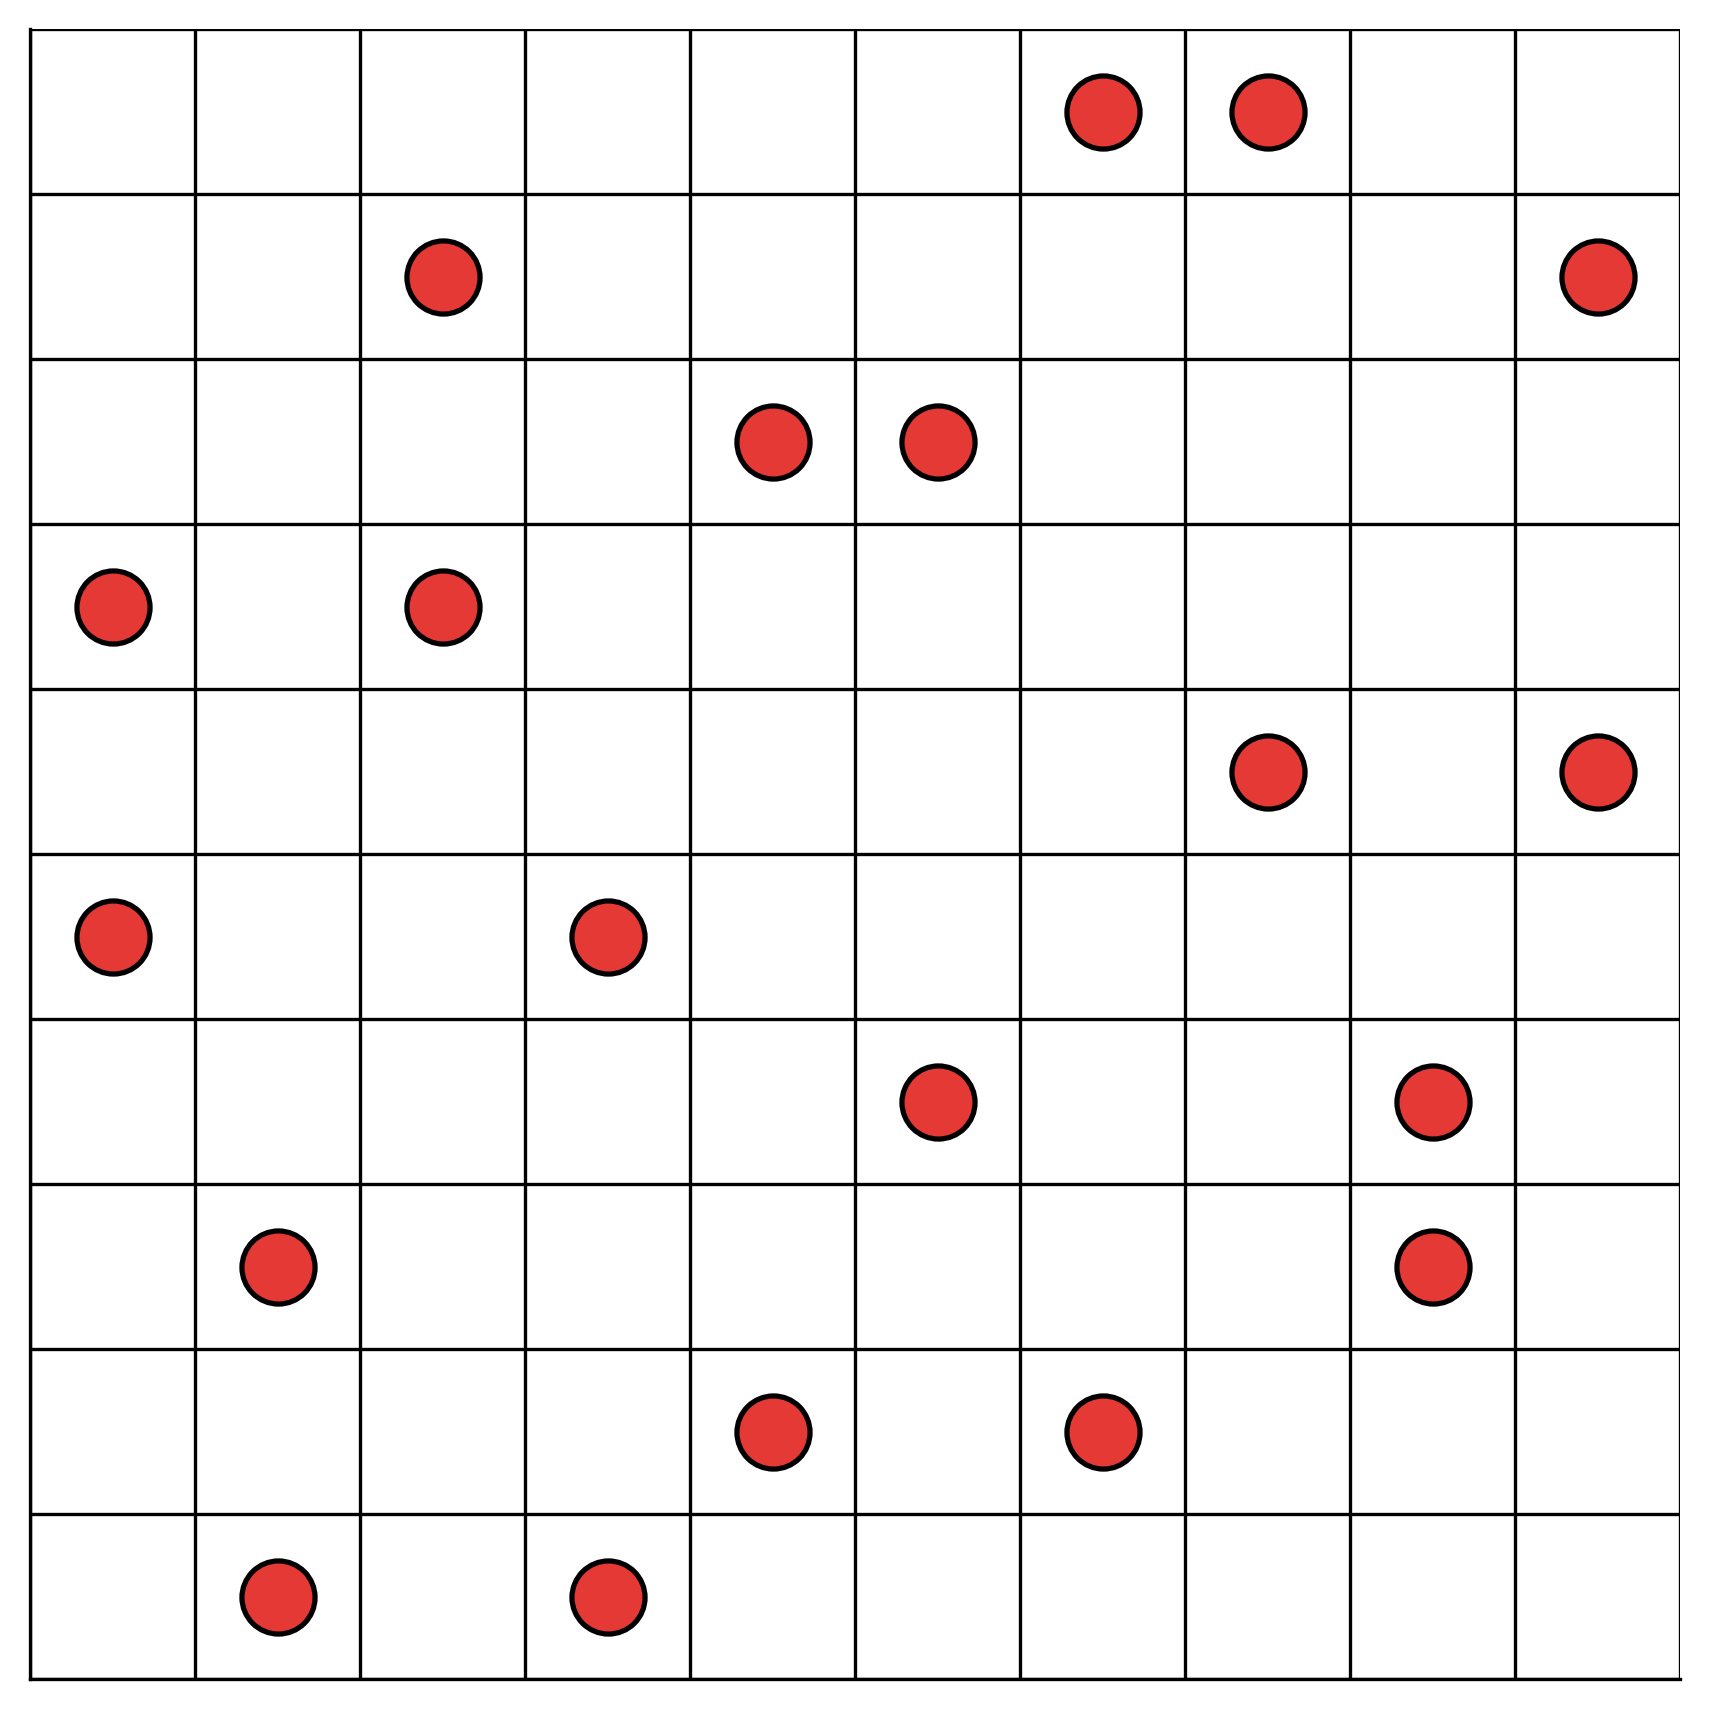
\includegraphics[width=0.72\linewidth]{no_three_in_line_n10.png}
\caption{Optimal solution for the No-Three-In-Line problem on a $10 \times 10$ grid, achieving the maximum of 20 points.}
\label{fig:problem_intro}
\end{figure}


A trivial upper bound of $2n$ points follows from the pigeonhole principle, as no row or column can contain more than two points. The first non-trivial lower bound was established by Paul Erd{\H{o}}s, who used modular parabola constructions to place approximately $n$ points \yrcite{ErdosRoth1951}. This was improved to approximately $1.5n$ by Hall, Jackson, Sudbery, and Wild using modular hyperbola constructions, which remains the best proven lower bound \yrcite{Hall1975}. Exact solutions achieving $2n$ points have been found for all $n \leq 60$ (\textit{T.~Prellberg, private communication, 2026}). However, Guy and Kelly conjectured that for sufficiently large $n$, the maximum asymptotically approaches only $cn$ points, where $c \approx 1.814$ \yrcite{GuyKelly1968}. This leaves a significant gap between the best-proven result and the conjectured limit, underscoring the problem's persistent difficulty.

Traditional computational approaches, such as recursive backtracking algorithms and integer linear programming (ILP), frame the No-Three-In-Line problem as a constraint satisfaction task by encoding collinearity constraints algebraically and using branch-and-bound optimization \cite{NemhauserWolsey1988, Eppstein2018}. Early computational efforts by Flammenkamp employed exhaustive backtracking search with sophisticated pruning techniques, successfully determining optimal configurations up to $n = 52$ \yrcite{Flammenkamp2010}. These enumeration methods systematically explore the search space while eliminating symmetric equivalents and configurations that violate constraints, but computation time grows exponentially with $n$. Constraint-programming and GPU-based methods have since pushed the frontier further: Google's CP-SAT solver finds provably optimal $2n$-point solutions up to $n = 60$ \cite{Prellberg2026}, and GPU enumeration extends this to $n = 67$. However, both gains depend critically on symmetry pruning: with that restriction removed, unrestricted exact completeness in the public record stops near $n \approx 19$ \cite{FlammenkampRecords,Prellberg2026}.

Tsuchiya and Takefuji applied classical neural networks to the No-Three-In-Line problem in 1995 \yrcite{Tsuchiya1995}; modern ML approaches have not revisited the problem until recently. Recent ML approaches to combinatorial optimization include reinforcement learning, graph neural networks, and transformer-based pattern search \cite{Mazyavkina2021,Cappart2023,Vaswani2017}. A recent breakthrough came with PatternBoost \cite{Charton2024}, which discovered a counterexample to Graham and Harary's conjecture on hypercube subgraphs \cite{GrahamHarary1992}. While these applications demonstrate PatternBoost's effectiveness on geometric point placement problems with distance-based constraints, its application to collinearity-based constraints remains unexplored.

This study presents the first comparison of classical and AI-driven methods for the No-Three-In-Line problem. We compare four approaches: integer linear programming using the Gurobi solver, transformer-based pattern learning via the PatternBoost framework, reinforcement learning using Proximal Policy Optimization (PPO) \cite{Schulman2017}, and SciML \cite{RackauckasNie2017,Karniadakis2021}.

To go beyond discrete search, we recast the No-Three-In-Line problem as continuous energy minimisation and solve it via gradient flow \cite{RackauckasNie2017,Karniadakis2021}. An energy that penalises collinearity and rewards point count drives placement variables in $[0,1]^{n^2}$ towards near-binary configurations, which are then thresholded to yield discrete solutions.

\textbf{Our contributions are:}
\begin{itemize}
    \item A novel SciML method that recasts the No-Three-In-Line problem as continuous energy minimisation and solves it via gradient flow on commodity GPU hardware without symmetry pruning.
    \item The first application of PatternBoost \cite{Charton2024} to a collinearity-constrained geometric problem.
    \item A PPO reinforcement-learning agent \cite{Schulman2017} with action masking, characterising both where reinforcement learning succeeds and how it fails under tight collinearity constraints.
\end{itemize}

\subsection{Problem Formulation}

The No-Three-In-Line problem is defined on an $n \times n$ discrete grid, where each cell $(i,j)$ with $0 \leq i,j < n$ represents a potential point placement. We represent a configuration as a binary matrix $\mathbf{X} \in \{0,1\}^{n \times n}$, where $x_{i,j} = 1$ indicates a point is placed at position $(i,j)$, and $x_{i,j} = 0$ indicates an empty cell.

\textbf{Collinearity Constraint.} Three distinct points $(x_1, y_1)$, $(x_2, y_2)$, and $(x_3, y_3)$ are collinear if and only if they satisfy:
\begin{equation}
\begin{vmatrix}
x_1 & y_1 & 1 \\
x_2 & y_2 & 1 \\
x_3 & y_3 & 1
\end{vmatrix} = 0
\end{equation}

This determinant evaluates to zero when the three points lie on a common line (horizontal, vertical, or diagonal). The constraint applies to \textit{all} possible straight lines passing through the grid, including lines with arbitrary rational slopes.

\textbf{Optimization Objective and Constraints.} With decision variables $x_{i,j} \in \{0,1\}$ indicating a point at $(i,j)$, the ILP formulation is:
\begin{align}
\max_{x_{i,j} \in \{0,1\}} \quad & \sum_{i=0}^{n-1} \sum_{j=0}^{n-1} x_{i,j} \\
\text{s.t.} \quad & \sum_{(i,j) \in \ell} x_{i,j} \le 2 \quad \forall \text{ grid lines } \ell \text{ with } |\ell| \ge 3.
\end{align}
Equivalently, the line constraint can be written for every triple of distinct grid points whose determinant above is zero:
\begin{equation}
\begin{split}
x_{i_1,j_1} + x_{i_2,j_2} + x_{i_3,j_3} \le 2 \quad \forall \text{ distinct } (i_k, j_k) \\
\text{such that }
\begin{vmatrix}
i_1 & j_1 & 1 \\
i_2 & j_2 & 1 \\
i_3 & j_3 & 1
\end{vmatrix}
= 0.
\end{split}
\end{equation}

\textbf{Constraint Enumeration.} For an $n \times n$ grid, there are $n^2$ grid cells, yielding $\binom{n^2}{3} = O(n^6)$ possible triplets of points. However, not all triplets lie on a common line. The number of \textit{collinear} triplets is $O(n^3)$, corresponding to all possible lines (defined by slope and intercept) that pass through at least three grid points. This determines the number of active constraints in the optimization problem.

This formulation establishes the combinatorial and geometric foundation upon which all subsequent methods are built.

\subsection{Integer Linear Programming}

We solve the No-Three-In-Line problem using integer linear programming (ILP) with the Gurobi Optimizer \cite{GurobiOptimization2024}. Using the formulation from Section 2.1, the implementation focuses on efficient constraint generation and solver configuration.

\textbf{Constraint Generation.} To enforce the no-three-in-line requirement, we enumerate collinear point sets as formalized in Algorithm~\ref{alg:ilp_constraints}.
\begin{algorithm}[htbp]
\caption{ILP Constraint Generation}
\label{alg:ilp_constraints}
\begin{algorithmic}[1]
\STATE {\bfseries Input:} Grid size $n$
\STATE {\bfseries Output:} Set of linear constraints $\mathcal{C}$
\STATE Initialize $\mathcal{C} \gets \emptyset$, line dictionary $\mathcal{L} \gets \{\}$
\FOR{each pair of distinct grid points $(i_1, j_1)$ and $(i_2, j_2)$}
    \STATE Compute line equation $ax + by + c = 0$ through both points
    \STATE Normalize: $(a, b, c) \gets (a, b, c) / \gcd(|a|, |b|, |c|)$
    \STATE Apply consistent sign convention to obtain canonical form $\ell$
    \IF{$\ell \notin \mathcal{L}$}
        \STATE $\mathcal{L}[\ell] \gets \emptyset$
    \ENDIF
    \STATE $\mathcal{L}[\ell] \gets \mathcal{L}[\ell] \cup \{(i_1, j_1), (i_2, j_2)\}$
\ENDFOR
\FOR{each line $\ell \in \mathcal{L}$ with $|\mathcal{L}[\ell]| \geq 3$}
    \STATE Add constraint: $\sum_{(i,j) \in \mathcal{L}[\ell]} x_{i,j} \leq 2$ to $\mathcal{C}$
\ENDFOR
\STATE {\bfseries Output:} $\mathcal{C}$
\end{algorithmic}
\end{algorithm}

\textbf{Implementation.} The resulting ILP model contains $n^2$ binary variables and $O(n^3)$ linear constraints, corresponding to the number of distinct lines passing through at least three grid points. We solve the model using Gurobi's branch-and-bound algorithm \cite{NemhauserWolsey1988} with default settings for cutting planes and primal heuristics.


\subsection{PatternBoost Transformer Learning}

We apply the PatternBoost methodology \cite{Charton2024} to the No-Three-In-Line problem, using a transformer to learn patterns from high-quality configurations and guide the search toward better solutions.

\textbf{Grid Representation and Tokenization.} Each $n \times n$ grid configuration is encoded as a sequence of tokens for transformer input. We map each grid cell $(i,j)$ to a unique integer token $t_{i,j} = i \cdot n + j \in \{0, 1, \ldots, n^2-1\}$. A configuration containing points at positions $\mathcal{P} = \{(i_1, j_1), (i_2, j_2), \ldots, (i_k, j_k)\}$ is represented as the sequence of tokens $(t_{i_1,j_1}, t_{i_2,j_2}, \ldots, t_{i_k,j_k})$. Each token corresponds to a single grid cell, yielding a vocabulary of size $n^2$. We prepend a special start token to each sequence.

\textbf{Transformer Architecture.} We employ a GPT-2 style decoder-only transformer \cite{Radford2019} based on Karpathy's Makemore implementation \cite{Karpathy2024}. The model consists of 4 transformer layers with 4 attention heads and a hidden dimension of 64. The feedforward network in each layer expands to dimension 256 ($4 \times$ hidden dimension) with GELU activation \cite{Hendrycks2023}. Token embeddings and learned positional embeddings are summed before processing through the transformer layers. The model performs next-token prediction via cross-entropy loss over the vocabulary. Figure \ref{fig:transformer_architecture} illustrates the complete architecture with residual connections between layers.

\begin{figure}[htbp]
	\centering
	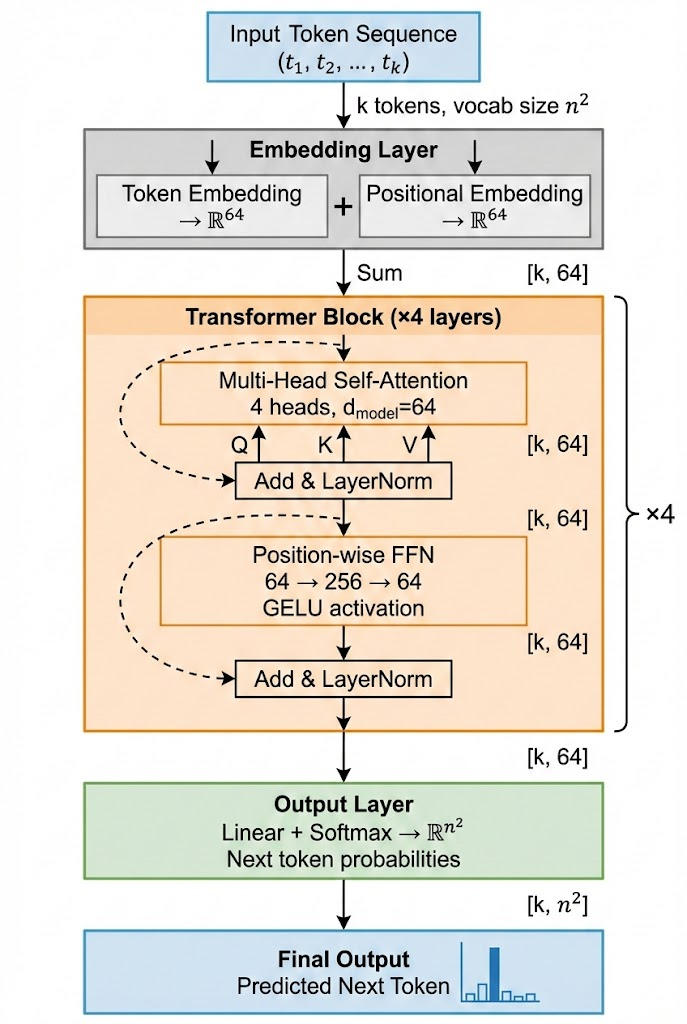
\includegraphics[width=\linewidth]{transformer.png}
	\caption{PatternBoost transformer: 4 layers, 4 heads, dimension 64, with residual connections.}
	\label{fig:transformer_architecture}
\end{figure}

\textbf{Training Data Generation.} Initial training data is generated via greedy saturation from the empty grid, formalized in Algorithm~\ref{alg:greedy_saturation}.
\begin{algorithm}[htbp]
\caption{Greedy Saturation for Training Data Generation}
\label{alg:greedy_saturation}
\begin{algorithmic}[1]
\STATE {\bfseries Input:} Empty $n \times n$ grid
\STATE {\bfseries Output:} Saturated configuration with no valid moves remaining
\STATE Initialize grid $G \gets \emptyset$ (all cells empty)
\WHILE{valid placements exist}
    \STATE $\mathcal{C} \gets \{(i,j) : G[i,j] = 0\}$ \COMMENT{All empty cells}
    \FOR{each candidate $(i,j) \in \mathcal{C}$}
        \STATE Simulate placing point at $(i,j)$
        \STATE Update forbidden regions based on collinearity constraints
        \STATE $\text{score}[i,j] \gets |\text{remaining available cells}|$
    \ENDFOR
    \STATE $(i^*, j^*) \gets \arg\max_{(i,j) \in \mathcal{C}} \text{score}[i,j]$ \COMMENT{Ties broken randomly}
    \STATE Place point at $(i^*, j^*)$ in $G$: $G[i^*, j^*] \gets 1$
\ENDWHILE
\STATE {\bfseries Output:} $G$
\end{algorithmic}
\end{algorithm}
This greedy lookahead strategy produces saturated configurations. We generate 20,000 such configurations in batches of 500, forming the initial training pool.

\textbf{Priority Queue (TopPool).} Best configurations are maintained in a fixed-capacity priority queue implemented as a min-heap of size $K = 20{,}000$. Each entry stores a tuple $(s, \sigma)$ where $s$ is the configuration score (number of points) and $\sigma$ is the tokenized sequence. When the heap is full and a new configuration with score $s' > s_{\min}$ arrives, the minimum-score entry is evicted and the new entry is inserted. This ensures training always uses the top-performing configurations discovered.

\textbf{Iterative Refinement Loop.} PatternBoost alternates between local and global optimization over 20 generations, formalized in Algorithm~\ref{alg:patternboost}.
\begin{algorithm}[htbp]
\caption{PatternBoost Iterative Refinement}
\label{alg:patternboost}
\begin{algorithmic}[1]
\STATE {\bfseries Input:} Initial pool $\mathcal{P}_0$ of 20,000 configurations, number of generations $T = 20$
\STATE {\bfseries Output:} Optimized configuration pool $\mathcal{P}_T$
\FOR{generation $t = 1$ to $T$}
    \STATE \textbf{Load Pool:} Initialize TopPool with $\mathcal{P}_{t-1}$
    \STATE \textbf{Data Augmentation:} $\mathcal{D}_t \gets \emptyset$
    \FOR{each configuration $c \in \mathcal{P}_{t-1}$}
        \STATE Generate all 8 symmetries (4 rotations $\times$ 2 reflections)
        \STATE Apply canonical form deduplication
        \STATE Add augmented configurations to $\mathcal{D}_t$
    \ENDFOR
    \STATE \textbf{Train Transformer:} Train model $\theta_t$ for 5,000 steps on $\mathcal{D}_t$ using AdamW \cite{Loshchilov2019} with cross-entropy loss
    \STATE \textbf{Generate Candidates:} Sample 20,000 token sequences $\{\sigma_1, \ldots, \sigma_{20000}\}$ from trained model $\pi_{\theta_t}$
    \FOR{each sequence $\sigma_i$, $i = 1$ to $20000$}
        \STATE \textbf{Decode:} Convert token sequence $\sigma_i$ to grid coordinates
        \STATE \textbf{Greedy Saturation:} Apply Algorithm~\ref{alg:greedy_saturation} to complete partial configuration
        \STATE \textbf{Evaluate:} Compute score $s_i$ (number of points placed)
        \STATE Attempt to insert $(s_i, \sigma_i)$ into TopPool (min-heap with capacity 20,000)
    \ENDFOR
    \STATE \textbf{Save Generation:} Persist updated pool $\mathcal{P}_t$ to disk
\ENDFOR
\STATE {\bfseries Output:} $\mathcal{P}_T$
\end{algorithmic}
\end{algorithm}

Table \ref{tab:patternboost_hyperparams} summarizes the complete hyperparameter configuration.

% training params
% architecture params
% gen params not required
\begin{table}[htbp]
\vspace{0.1in}
\begin{center}
\begin{small}
\begin{sc}
\caption{PatternBoost Hyperparameters}
\label{tab:patternboost_hyperparams}
\resizebox{\columnwidth}{!}{%
\begin{tabular}{ll}
\toprule
\textbf{Parameter} & \textbf{Value} \\
\midrule
\multicolumn{2}{l}{\textup{Transformer Architecture}} \\
Layers & 4 \\
Attention heads & 4 \\
Hidden dimension & 64 \\
Feedforward dimension & 256 \\
Activation function & GELU \\
Loss function & Cross-entropy \\
\midrule
\multicolumn{2}{l}{\textup{Training Configuration}} \\
Optimizer & AdamW \\
Learning rate & $10^{-4}$ \\
Weight decay & 0.1 \\
Batch size & 64 \\
% Steps per generation & 5,000 \\
% Number of generations & 20 \\
% Train/test split & 90/10 \\
% Checkpoint frequency & Every 500 steps \\
\bottomrule
\end{tabular}}
\end{sc}
\end{small}
\end{center}
\vspace{0.1in}
\end{table}

%  span the entire rest of page

\textbf{Symmetry Handling.} To increase training data diversity and prevent redundant storage, we apply symmetry processing at two stages. During data augmentation, each configuration is expanded to all 8 symmetric versions (4 rotations and 2 reflection states), increasing the training dataset size by $8\times$. When inserting into TopPool, configurations are mapped to their lexicographically smallest canonical form under these symmetries to prevent storing duplicate equivalent solutions. This approach maximizes training signal while maintaining pool diversity.

% \textbf{Implementation Details.} The model checkpoint is saved when test loss improves, and training continues from the previous checkpoint if available. We evaluate every 500 steps on a 90/10 train/test split. Sampling uses stochastic generation with temperature 1.0 and batch size 10. We track pre-saturation scores to assess transformer output quality before greedy completion. The complete training process runs for 20 generations.

\subsection{Proximal Policy Optimization Reinforcement Learning}

We formulate the No-Three-In-Line problem as a sequential decision-making task and solve it using deep reinforcement learning. We employ Proximal Policy Optimization (PPO) \cite{Schulman2017} with action masking to train agents that learn to place points on the grid while satisfying the collinearity constraint.

\subsubsection{Markov Decision Process Formulation}

The problem is modeled as a Markov Decision Process (MDP) \cite{Towers2024} with tuple $(\mathcal{S}, \mathcal{A}, P, R, \gamma)$. The state space $\mathcal{S}$ consists of $n \times n$ binary grids $s_t \in \{0,1\}^{n \times n}$, where $s_t(i,j) = 1$ indicates a placed point. The action space $\mathcal{A}$ is discrete with $|\mathcal{A}| = n^2$, and action $a = i \cdot n + j$ places a point at position $(i,j)$. We use action masking to restrict the agent to empty cells only. The transition function $P(s_{t+1}|s_t, a_t)$ is deterministic: choosing action $a_t$ sets $s_{t+1}(i,j) = 1$ at the selected location.

The reward function balances exploration with constraint satisfaction using sparse rewards and dense penalties:
\begin{equation}
R(s_t, a_t) = \begin{cases}
+1.0 & \text{valid placement} \\
-10 & \text{collinearity violation} \\
-1 & \text{occupied cell} \\
+100 & k = 2n,\ \mathrm{violations} = 0 \\
+10 & k = 2n,\ \mathrm{violations} > 0
\end{cases}
\end{equation}
where $k$ is the current number of placed points. The final two cases correspond to perfect completion and imperfect completion, respectively. The 10:1 penalty-to-reward ratio encourages constraint satisfaction over rapid point accumulation, while the large perfect solution bonus creates a strong gradient toward zero-violation configurations. We use discount factor $\gamma = 0.99$.

Collinearity is detected using the determinant formula: three points $(x_1, y_1)$, $(x_2, y_2)$, $(x_3, y_3)$ are collinear if $(x_2 - x_1)(y_3 - y_1) = (x_3 - x_1)(y_2 - y_1)$. For each new placement, we check all $\binom{k}{2}$ pairs of existing points. Episodes terminate when $k = 2n$ points are placed, with no early termination on violations to allow recovery from mistakes.

\subsubsection{PPO Algorithm and Network Architecture}

We employ Proximal Policy Optimization with action masking (MaskablePPO) from Stable-Baselines3 Contrib \cite{Raffin2021}. PPO optimizes a clipped surrogate objective:
\begin{equation}
\begin{aligned}
L^{\mathrm{CLIP}}(\theta) = \mathbb{E}_{t}\!\left[\min\!\bigl(r_t(\theta)\hat{A}_t,\right. \\
\qquad\left.\mathrm{clip}(r_t(\theta),1-\epsilon,1+\epsilon)\hat{A}_t\bigr)\right]
\end{aligned}
\end{equation}
where $r_t(\theta) = \frac{\pi_\theta(a_t|s_t)}{\pi_{\theta_{\text{old}}}(a_t|s_t)}$ is the probability ratio and $\epsilon = 0.2$ is the clipping parameter. The total loss combines the clipped objective with value function loss $L^{VF}(\theta) = (V_\theta(s_t) - V^{\text{target}}_t)^2$ and entropy bonus $S[\pi_\theta](s_t)$:
\begin{equation}
L_{\text{total}}(\theta) = L^{CLIP}(\theta) - c_1 L^{VF}(\theta) + c_2 S[\pi_\theta](s_t)
\end{equation}
with coefficients $c_1 = 0.5$ and $c_2 = 0.01$. Advantage estimates $\hat{A}_t$ are computed using Generalized Advantage Estimation (GAE) \cite{Schulman2016} with $\lambda = 0.95$ and $\gamma = 0.99$.

The policy network uses a multi-layer perceptron (MLP) with two hidden layers of 512 units each and ReLU activations. The architecture processes the flattened $n^2$-dimensional observation vector to produce action probabilities over the $n^2$ action space. The policy network (actor) $\pi_\theta(a|s)$ and value function (critic) $V_\theta(s)$ share feature extraction layers but have separate output heads, as shown in Figure \ref{fig:ppo_architecture}.

\begin{figure}[H]
		\centering
		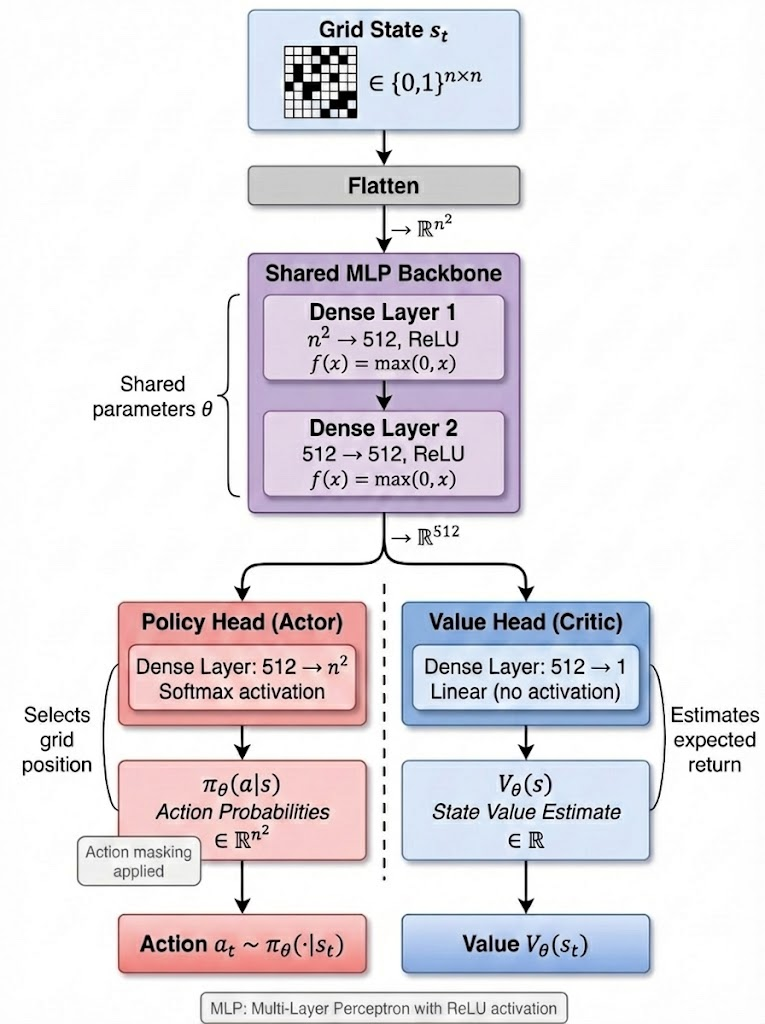
\includegraphics[width=\linewidth]{RL.png}
		\caption{PPO actor-critic with shared $512\times2$ MLP backbone splitting into policy and value heads.}
		\label{fig:ppo_architecture}
		\end{figure}

\subsubsection{Training Configuration}

We use the Adam optimizer \cite{Kingma2015} with learning rate $\alpha_0 = 3 \times 10^{-4}$ and exponential decay: $\alpha_t = \alpha_0 \cdot (0.8)^{\lfloor t / 10^6 \rfloor}$. Training employs 30 parallel environments, collecting 2048 steps per environment (61,440 total samples) before each policy update using batches of 1024 samples. The complete training runs for 10 epochs of 1,000,000 steps each (10,000,000 total steps). Table \ref{tab:ppo_hyperparams} summarizes the complete hyperparameter configuration.

\begin{table}[htbp]
\vspace{0.1in}
\begin{center}
\begin{small}
\begin{sc}
\caption{PPO Hyperparameters}
\label{tab:ppo_hyperparams}
\resizebox{\columnwidth}{!}{%
\begin{tabular}{ll}
\toprule
\textbf{Parameter} & \textbf{Value} \\
\midrule
Training epochs & 10 \\
Network architecture & [512, 512] MLP \\
Activation function & ReLU \\
Learning rate & $3 \times 10^{-4}$ \\
Optimizer & Adam ($\beta_1=0.9$, $\beta_2=0.999$) \\
GAE $\lambda$ & 0.95 \\
Discount $\gamma$ & 0.99 \\
PPO clip $\epsilon$ & 0.2 \\
Value coefficient $c_1$ & 0.5 \\
Entropy coefficient $c_2$ & 0.01 \\
\bottomrule
\end{tabular}}
\end{sc}
\end{small}
\end{center}
\vspace{0.1in}
\end{table}

Model performance is evaluated every epoch over 20 episodes using success rate (fraction achieving $2n$ points with zero violations), average violations, and a composite score that balances points placed, efficiency, and constraint satisfaction. The best model is selected based on maximum composite score across all training epochs.

\subsection{SciML Gradient Flow}
\label{sec:sciml}

% TODO(SciML): one-paragraph framing — discrete N3L recast as continuous
% relaxation x_{ij} in [0,1]^{n^2}; reformulate as energy-minimisation
% solved via gradient-flow ODE; mirror NeurIPS draft "Our Approach"
% paragraph. ~100 words. Cite RackauckasNie2017, Karniadakis2021.

\subsubsection{Continuous Relaxation and Energy Function}

% TODO(SciML): define E(x) = alpha * E_collinear + E_count + beta * E_binary
% (double-well 4x^2(1-x)^2). State sparse incidence matrix L reduces
% O(n^6) -> O(n^3). Cross-ref Section 2.1 problem formulation; do NOT
% repeat the determinant collinearity test. ~150 words + one equation.
% Source: NeurIPS_Paper/structure.txt section 3.1 + 3.2.

\subsubsection{Gradient Flow Dynamics}

% TODO(SciML): dx/dt = -grad E(x); RK4 integration on Apple Metal GPU;
% integration horizon T; optional two-stage ADAM -> LBFGS refinement.
% ~80 words. Source: NeurIPS_Paper/structure.txt section 3.3.

\subsubsection{Parallel Trajectory Search on Apple Metal}

% TODO(SciML): describe main_metal_v3.jl --- line-based custom Metal
% kernel v3, lock-free parallel trajectories (default 30), early-best
% heuristic (solutions emerge in first 10--20% of trajectory),
% threshold tau for continuous -> binary recovery. Cite Metal.jl.
% ~120 words. Source: experiments/main_metal_v3.jl + structure.txt 3.4.

\subsubsection{Hyperparameters and Parameter Scaling}

% TODO(SciML): hyperparameter table mirroring tab:patternboost_hyperparams
% / tab:ppo_hyperparams --- alpha, beta, gamma, T, n_traj, dt,
% integrator, optimiser stages, threshold tau. Note alpha scales
% linearly ~25--50 per unit n (NeurIPS draft section 3.5).
% Source: experiments/data/hyperparam_labels.csv.

\section{Results} % CHANGE (Frontiers): separate results from methods.


\subsection{Experimental Setup}

We evaluated each method across multiple grid sizes to assess solution quality and scalability. ILP was tested on grids up to $n = 19$, PatternBoost on grids up to $n = 15$, and PPO on grids up to $n = 11$. All experiments were conducted on an Apple M2 with 32 GB RAM. Software implementations used Python with PyTorch for neural network training, Gurobi for integer programming, and Stable-Baselines3 for reinforcement learning.

\subsection{Solution Quality and Scalability}

Table \ref{tab:results_comparison} presents the solution quality achieved by each method across different grid sizes. We report the maximum number of points successfully placed while satisfying the no-three-in-line constraint (zero violations). For reference, we include known optimal values $2n$ for grid size $n \times n$.

\begin{table}[htbp]
\vspace{0.1in}
\begin{center}
\begin{small}
\begin{sc}
\caption{Solution Quality Comparison Across Methods and Grid Sizes}
\label{tab:results_comparison}
% TODO(SciML): fill SciML column from
%   experiments/ablation/g1/metal_ablation_g1_10_to_18_summary.csv
%   experiments/ablation/g1/metal_ablation_g1_19_summary.csv
% Headline numbers (g1, mean-incidence, 10 runs/n):
%   n=10 10/10 (20),  n=11 7/10 (22 best, 1 viol fails),
%   n=12 10/10 (24),  n=13 8/10 (26),
%   n=14 4/10 (28),   n=15 8/10 (30),
%   n=16 8/10 (32),   n=17 0/10 (33 best, 1 viol),
%   n=18 9/10 (36),   n=19 0/10 (35 best, 3 viol).
% Decide whether to add new rows for n=11/13/16/17/18 (SciML tested
% there, ILP/PB/PPO not). For now table keeps original n list.
\resizebox{\columnwidth}{!}{%
\begin{tabular}{cccccc}
\toprule
\textbf{Grid Size} & \textbf{ILP} & \textbf{PatternBoost} & \textbf{PPO} & \textbf{SciML} & \textbf{Known Optimal} \\
\midrule
$5\times 5$   & 10 & 10 & 10 & -- & 10 \\ % TODO(SciML): n=5 not in ablation
$8\times 8$   & 16 & 16 & 16 & -- & 16 \\ % TODO(SciML): n=8 not in ablation
$10\times 10$ & 20 & 20 & 20 & 20 & 20 \\ % TODO(SciML): success-rate annotation 10/10
$12\times 12$ & 24 & 24 & -  & 24 & 24 \\ % TODO(SciML): success-rate annotation 10/10
$14\times 14$ & 28 & 28 & -  & 28 & 28 \\ % TODO(SciML): success-rate annotation 4/10
$15\times 15$ & 30 & 29 & -  & 30 & 30 \\ % TODO(SciML): success-rate annotation 8/10
$19\times 19$ & 38 & -  & -  & -- & 38 \\ % TODO(SciML): 0/10, best 35 (3 viol)
\bottomrule
\end{tabular}}
\end{sc}
\end{small}
\end{center}
\vspace{0.1in}
\end{table}

\textbf{Integer Linear Programming.} ILP using Gurobi achieved provably optimal solutions across all tested grid sizes, successfully scaling to $n = 19$ where it placed 38 points. The branch-and-bound algorithm with constraint pruning enables exact optimization for grids where the $O(n^3)$ constraint space remains tractable. ILP provides the strongest baseline, demonstrating that traditional optimization methods remain highly effective for well-structured combinatorial problems. Figure \ref{fig:ilp_n19} shows the optimal $19 \times 19$ configuration, illustrating the complex geometric structure required for maximum point placement while satisfying all collinearity constraints.

\textbf{PatternBoost.} The transformer-based approach achieved optimal solutions on grids up to $n = 14$ (28 points), matching known optimal values despite never observing optimal training examples. On $n = 15$ grids, PatternBoost discovered 29-point configurations, demonstrating modest generalization beyond its training distribution. The method successfully learned to recombine geometric patterns from greedy-generated examples, achieving competitive performance without exhaustive search. However, PatternBoost did not scale beyond $n = 15$, suggesting limitations in pattern generalization for larger grid sizes. The training dynamics presented in Section 3.3 reveal how iterative refinement and pattern learning enable this performance through progressive improvement across 20 generations.

\textbf{Proximal Policy Optimization.} PPO achieved perfect solutions on $n = 10$ grids (20 points with zero violations), successfully learning valid placement policies through reward-based feedback. On $n = 11$ grids, the agent placed 22 points but incurred a single collinearity violation, indicating difficulty maintaining long-term constraint satisfaction as problem complexity increases. PPO demonstrated the ability to discover effective strategies from minimal problem structure (only the reward signal), but struggled to scale beyond small grid sizes where sequential planning becomes critical. Figures \ref{fig:rl_success} and \ref{fig:rl_failure} illustrate this sharp performance transition between successful constraint satisfaction at $n = 10$ and systematic failure at $n = 11$, with detailed analysis of failure modes provided in Section 3.4.

\textbf{SciML.} % TODO(SciML): ~150 words. Headline: optimal 2n recovered
% for n = 10..16 and n = 18 on Apple M2 Metal, without symmetry pruning;
% failure modes at n = 17 (0/10 success, best config has 1 violation)
% and n = 19 (0/10, best config has 3 violations). Mention Metal-GPU
% runtime at headline n: e.g. n=18 ~588 s mean solver elapsed.
% Cross-ref Fig:sciml_solution_n18 and Fig:sciml_alpha_scaling.
% Source: experiments/ablation/g1/metal_ablation_g1_*_summary.csv.

% TODO(SciML): figure --- best 36-point n=18 SciML solution.
% Path: figures/sciml_solution_n18.png  (NOT YET COPIED IN).
% Source: /Users/pranavr/Developer/Work/Research/neurIPS/NeurIPS_Paper/
%         experiments/solutions_ablation/g1/  (best n=18 run).
% Mirror existing fig:patternboost_n14 / fig:ilp_n19 layout.

\subsection{Training Dynamics}

Figure \ref{fig:patternboost_loss} shows PatternBoost's loss over 15,000 training steps. Training loss rapidly decreases from 5.5 to below 0.5 within the first 2,000 steps, demonstrating effective pattern learning from greedy-generated configurations. Test loss follows a similar trajectory, initially dropping from 3.0 to 0.5 by step 2,000, achieving a 96\% reduction over the training period. The minimal train-test gap throughout training indicates strong generalization without overfitting, confirming that the transformer successfully learns reusable geometric patterns rather than memorizing training examples. The small spike in test loss around step 12,000 corresponds to a generation transition where the training pool was updated with higher-quality configurations, temporarily increasing task difficulty before the model adapted. By the final generation, both train and test losses stabilize near 0.1, indicating convergence to patterns that reliably predict valid point placements.

\begin{figure}[htbp]
		\centering
		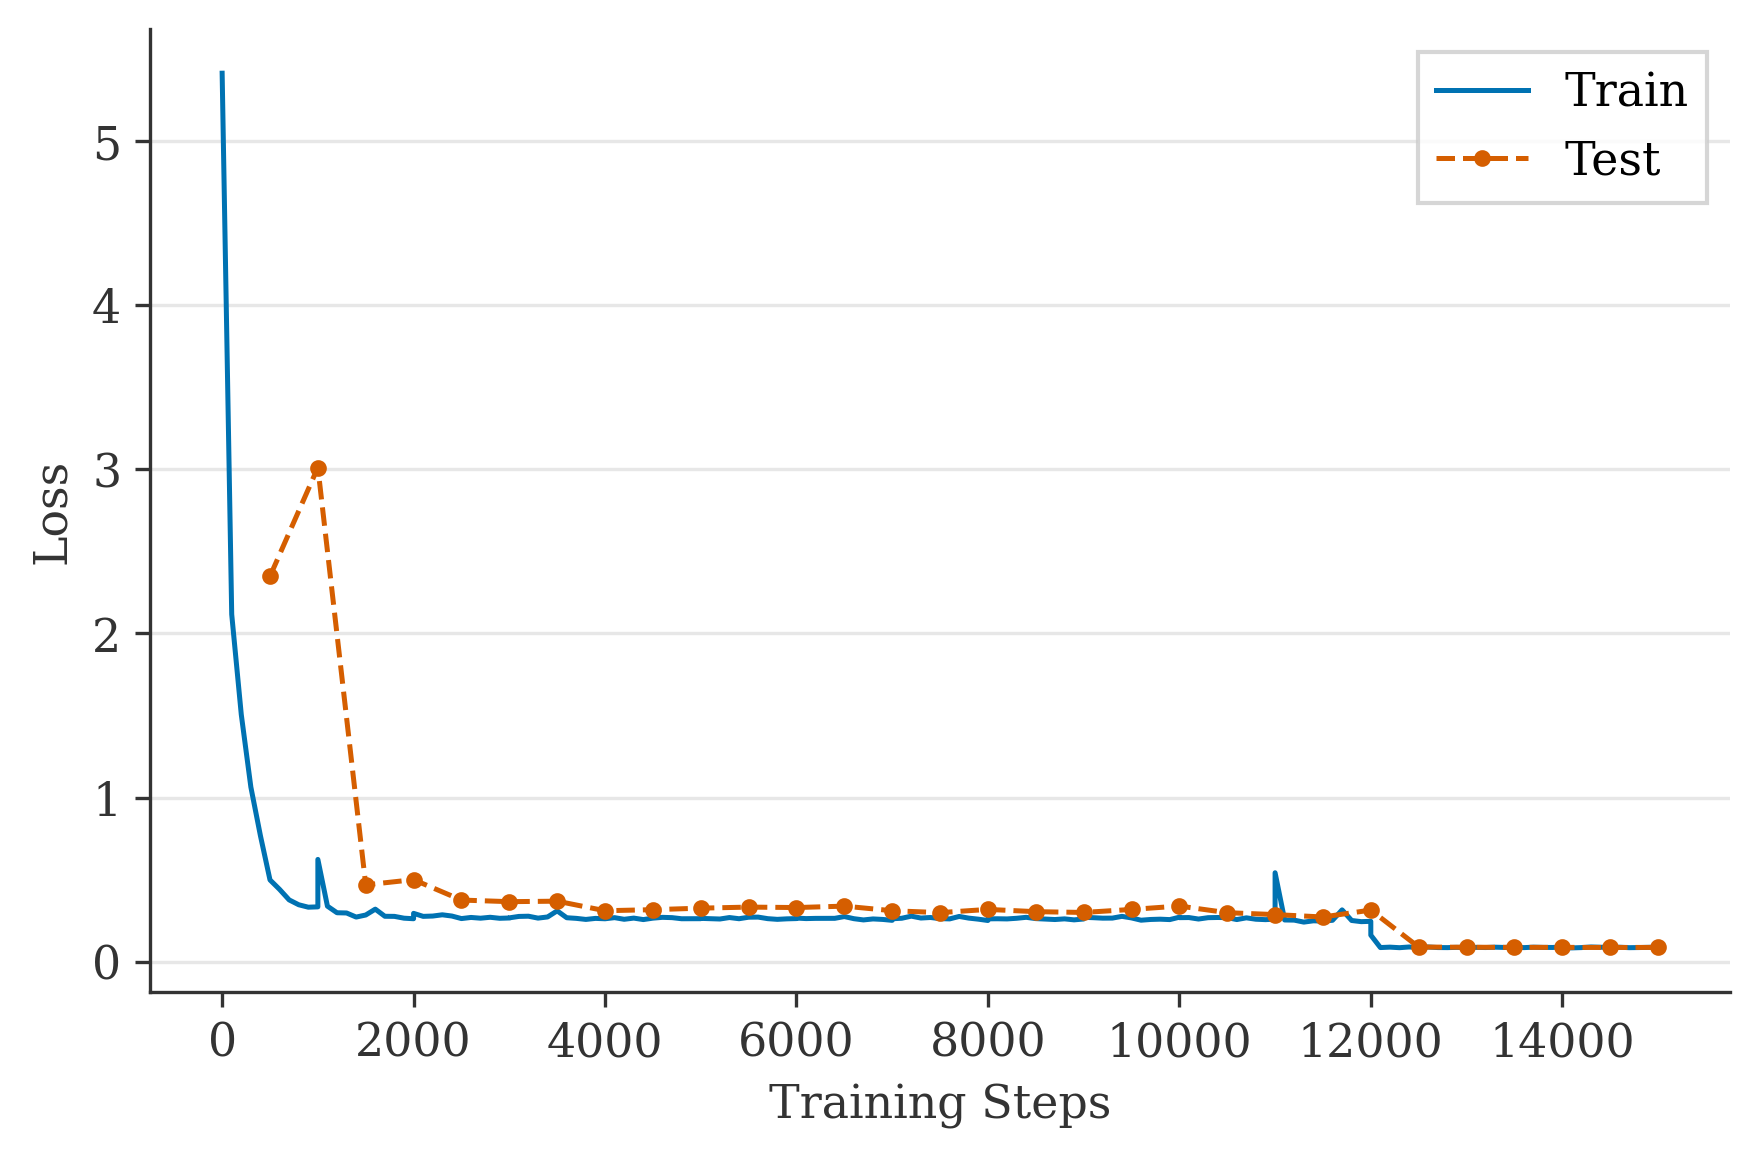
\includegraphics[width=\linewidth]{loss_plot.png}
		\caption{PatternBoost training and test loss over 15,000 steps.}
		\label{fig:patternboost_loss}
\end{figure}

\subsection{Parameter Scaling for SciML}

% TODO(SciML): describe alpha (collinearity penalty) scaling with n.
% Empirical observation: alpha grows ~25--50 per unit n
% (NeurIPS draft section 3.5). Source CSV:
%   experiments/ablation/g1/metal_ablation_g1_10_to_18.csv
% (per-run alpha column). ~120 words + scaling-laws figure.

% TODO(SciML): figure --- alpha vs n scaling plot.
% Path: figures/sciml_alpha_scaling.png  (NOT YET COPIED IN).
% Source: regenerate from experiments/data/hyperparam_labels.csv.
% Mirror layout/sizing of fig:patternboost_loss.

% TODO(SciML): convergence-trajectory figure (energy(t) trace) showing
% the early-best heuristic --- solutions emerge in first 10--20% of
% trajectory.  Path: figures/sciml_trajectory.png (NOT YET COPIED IN).
% Source: experiments/results_ablation/logs_20260423_224700/.

\subsection{Limitations}

Figures \ref{fig:rl_success} and \ref{fig:rl_failure} illustrate PPO's performance transition between successful and failed constraint satisfaction. On $10 \times 10$ grids (Figure \ref{fig:rl_success}), the agent consistently achieves perfect solutions with 20 points and zero violations, demonstrating successful policy learning for problems of this scale. However, on $11 \times 11$ grids (Figure \ref{fig:rl_failure}), despite placing 22 points, the agent incurs a single collinearity violation (highlighted point in red box), revealing the brittleness of learned policies as problem complexity increases. The violation occurs in a densely populated region where multiple collinearity constraints intersect, suggesting that the policy network struggles to maintain global constraint awareness when the number of placed points exceeds approximately 20. This represents a sharp transition from reliable performance to systematic failure as grid size increases by just one row and column.

PatternBoost's failure at $n = 15$ follows a different pattern. While achieving 29 points on $15 \times 15$ grids, one point short of the known optimum of 30, the method demonstrates graceful degradation rather than catastrophic failure. The configurations discovered remain valid (zero violations) but fail to reach optimality, suggesting that the transformer's learned patterns generalize approximately but not perfectly to larger grids. Figure \ref{fig:patternboost_n14} shows PatternBoost's optimal $14 \times 14$ solution achieving 28 points, demonstrating the geometric patterns successfully learned through iterative refinement. Figure \ref{fig:ilp_n19} shows ILP's optimal $19 \times 19$ solution for comparison, illustrating the increased complexity that AI methods must learn to replicate at larger scales.

\begin{figure}[htbp]
		\centering
		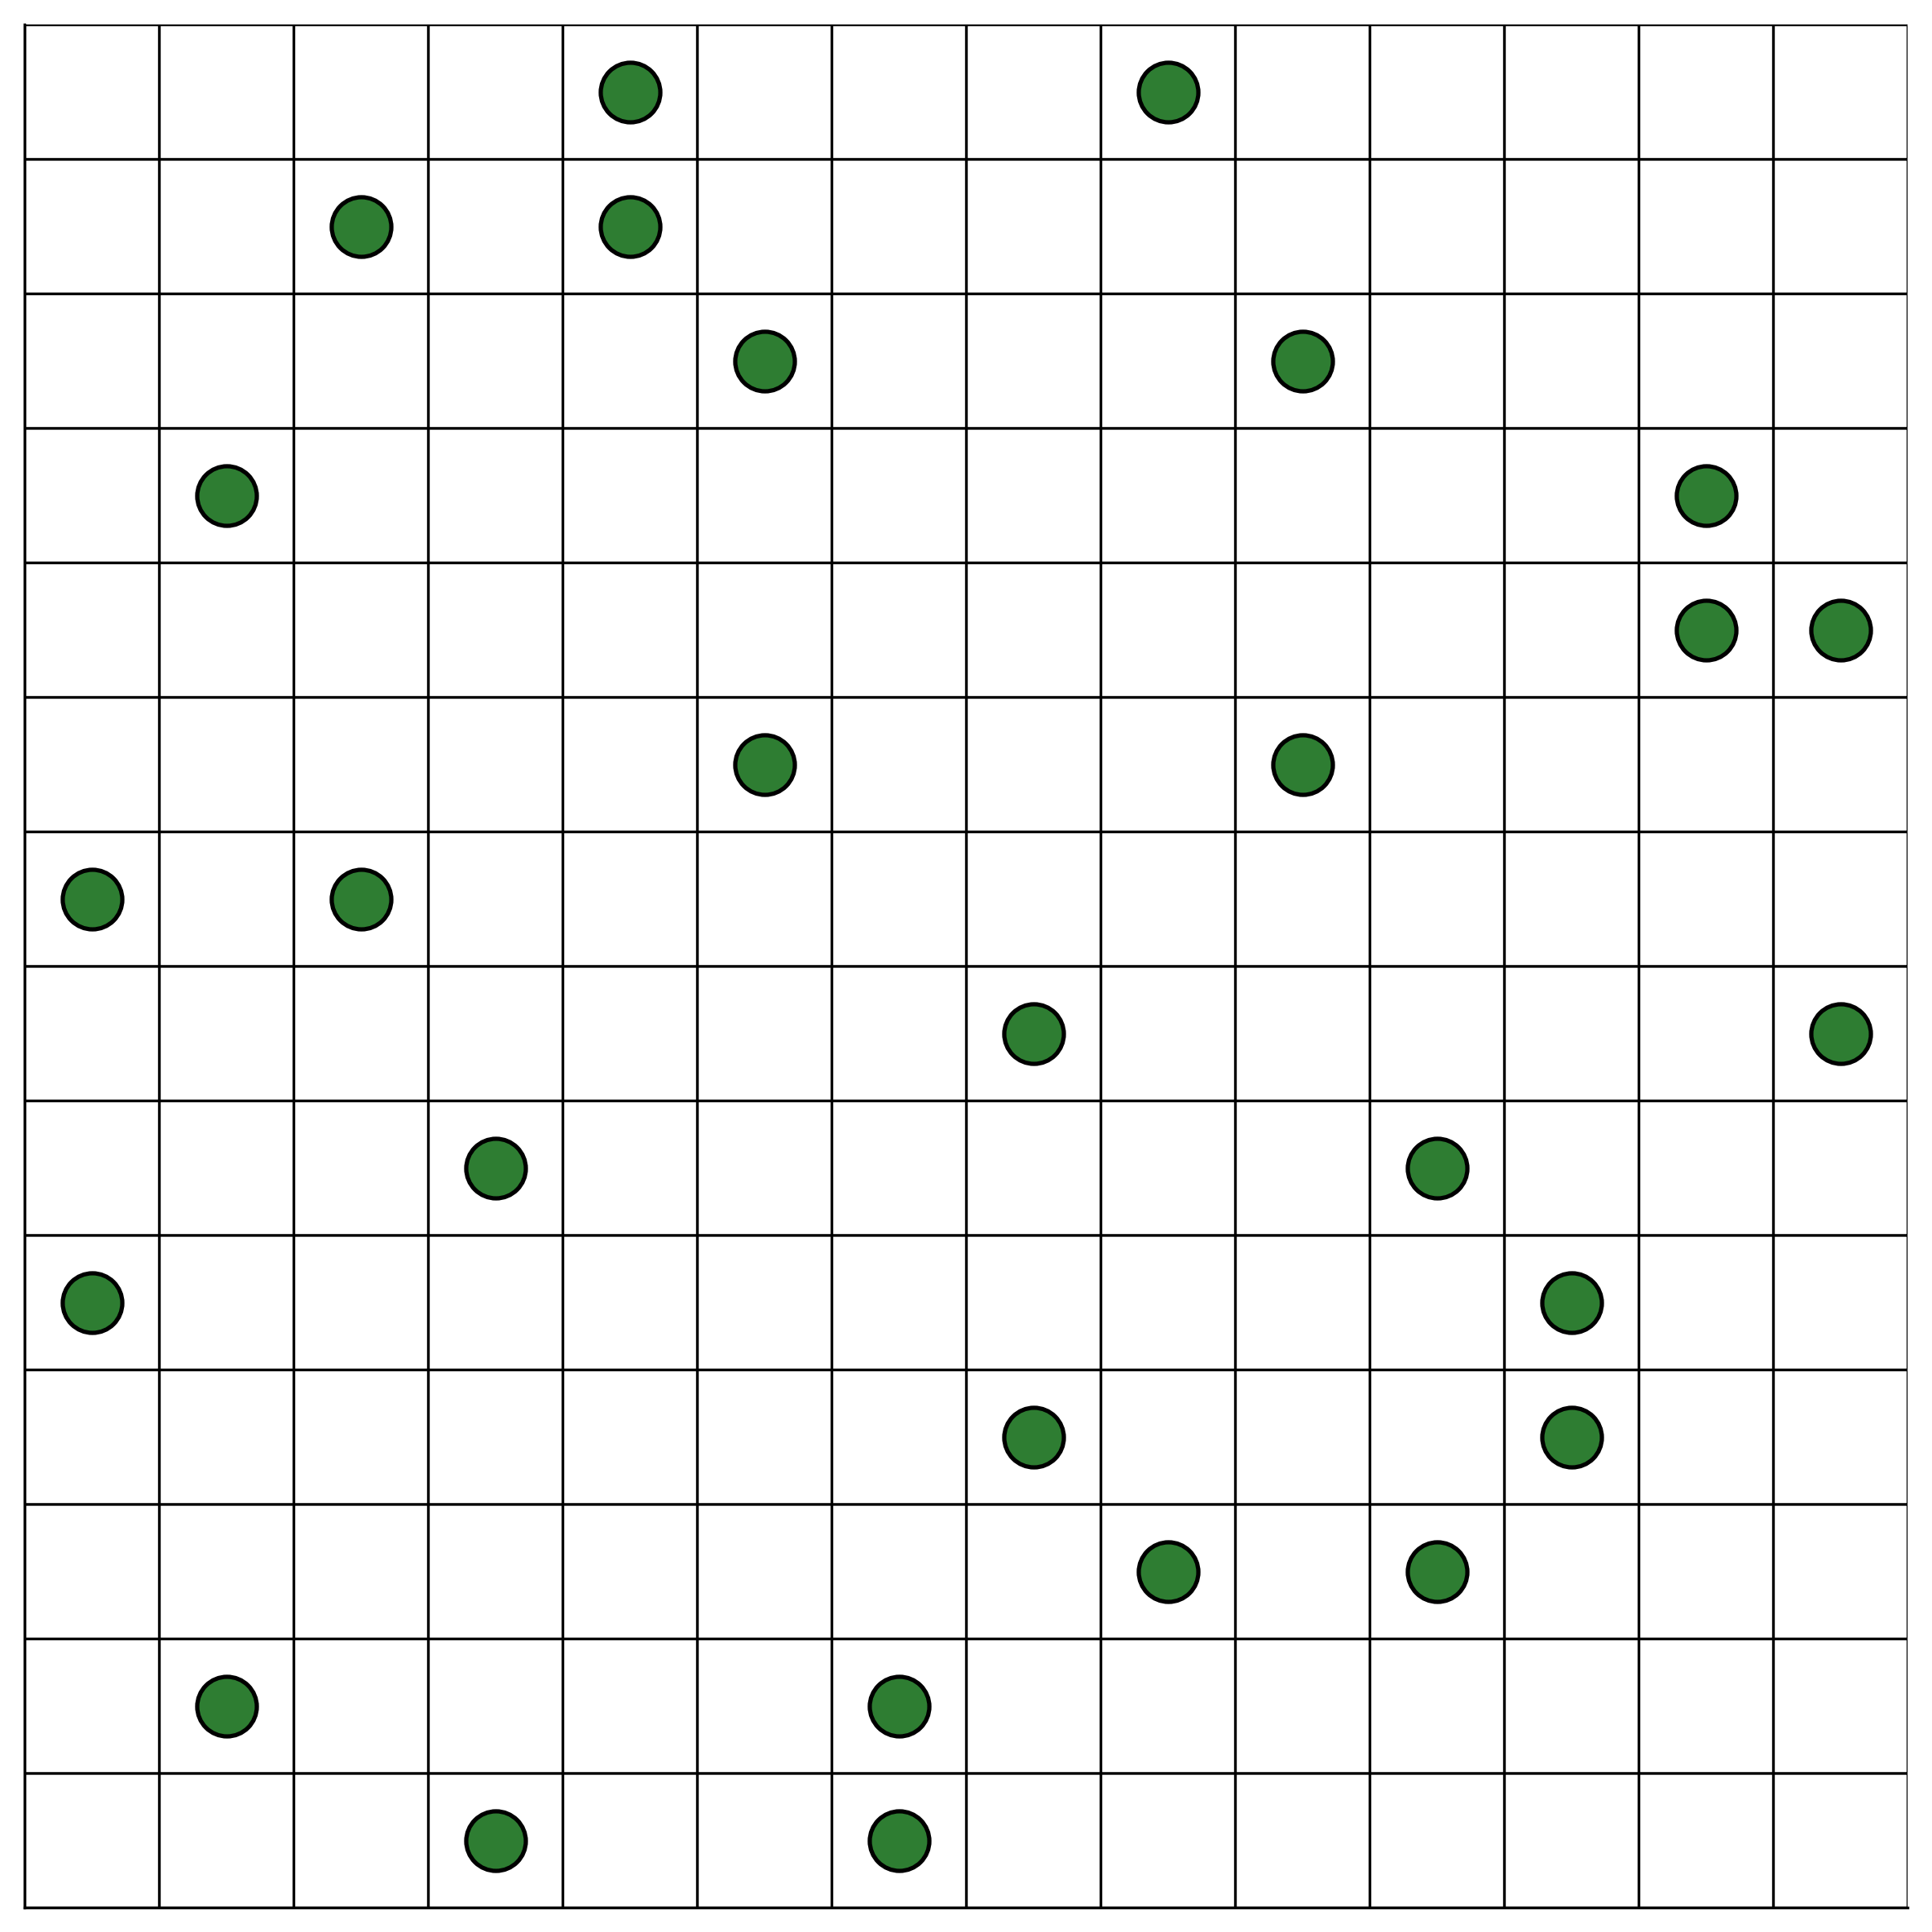
\includegraphics[width=\linewidth]{PatternBoost_n14.png}
		\caption{PatternBoost optimal solution on $14 \times 14$ grid achieving 28 points, demonstrating successful pattern learning from greedy-generated training data.}
		\label{fig:patternboost_n14}
\end{figure}

\begin{figure}[htbp]
	\centering
	\begin{minipage}{0.48\textwidth}
		\centering
		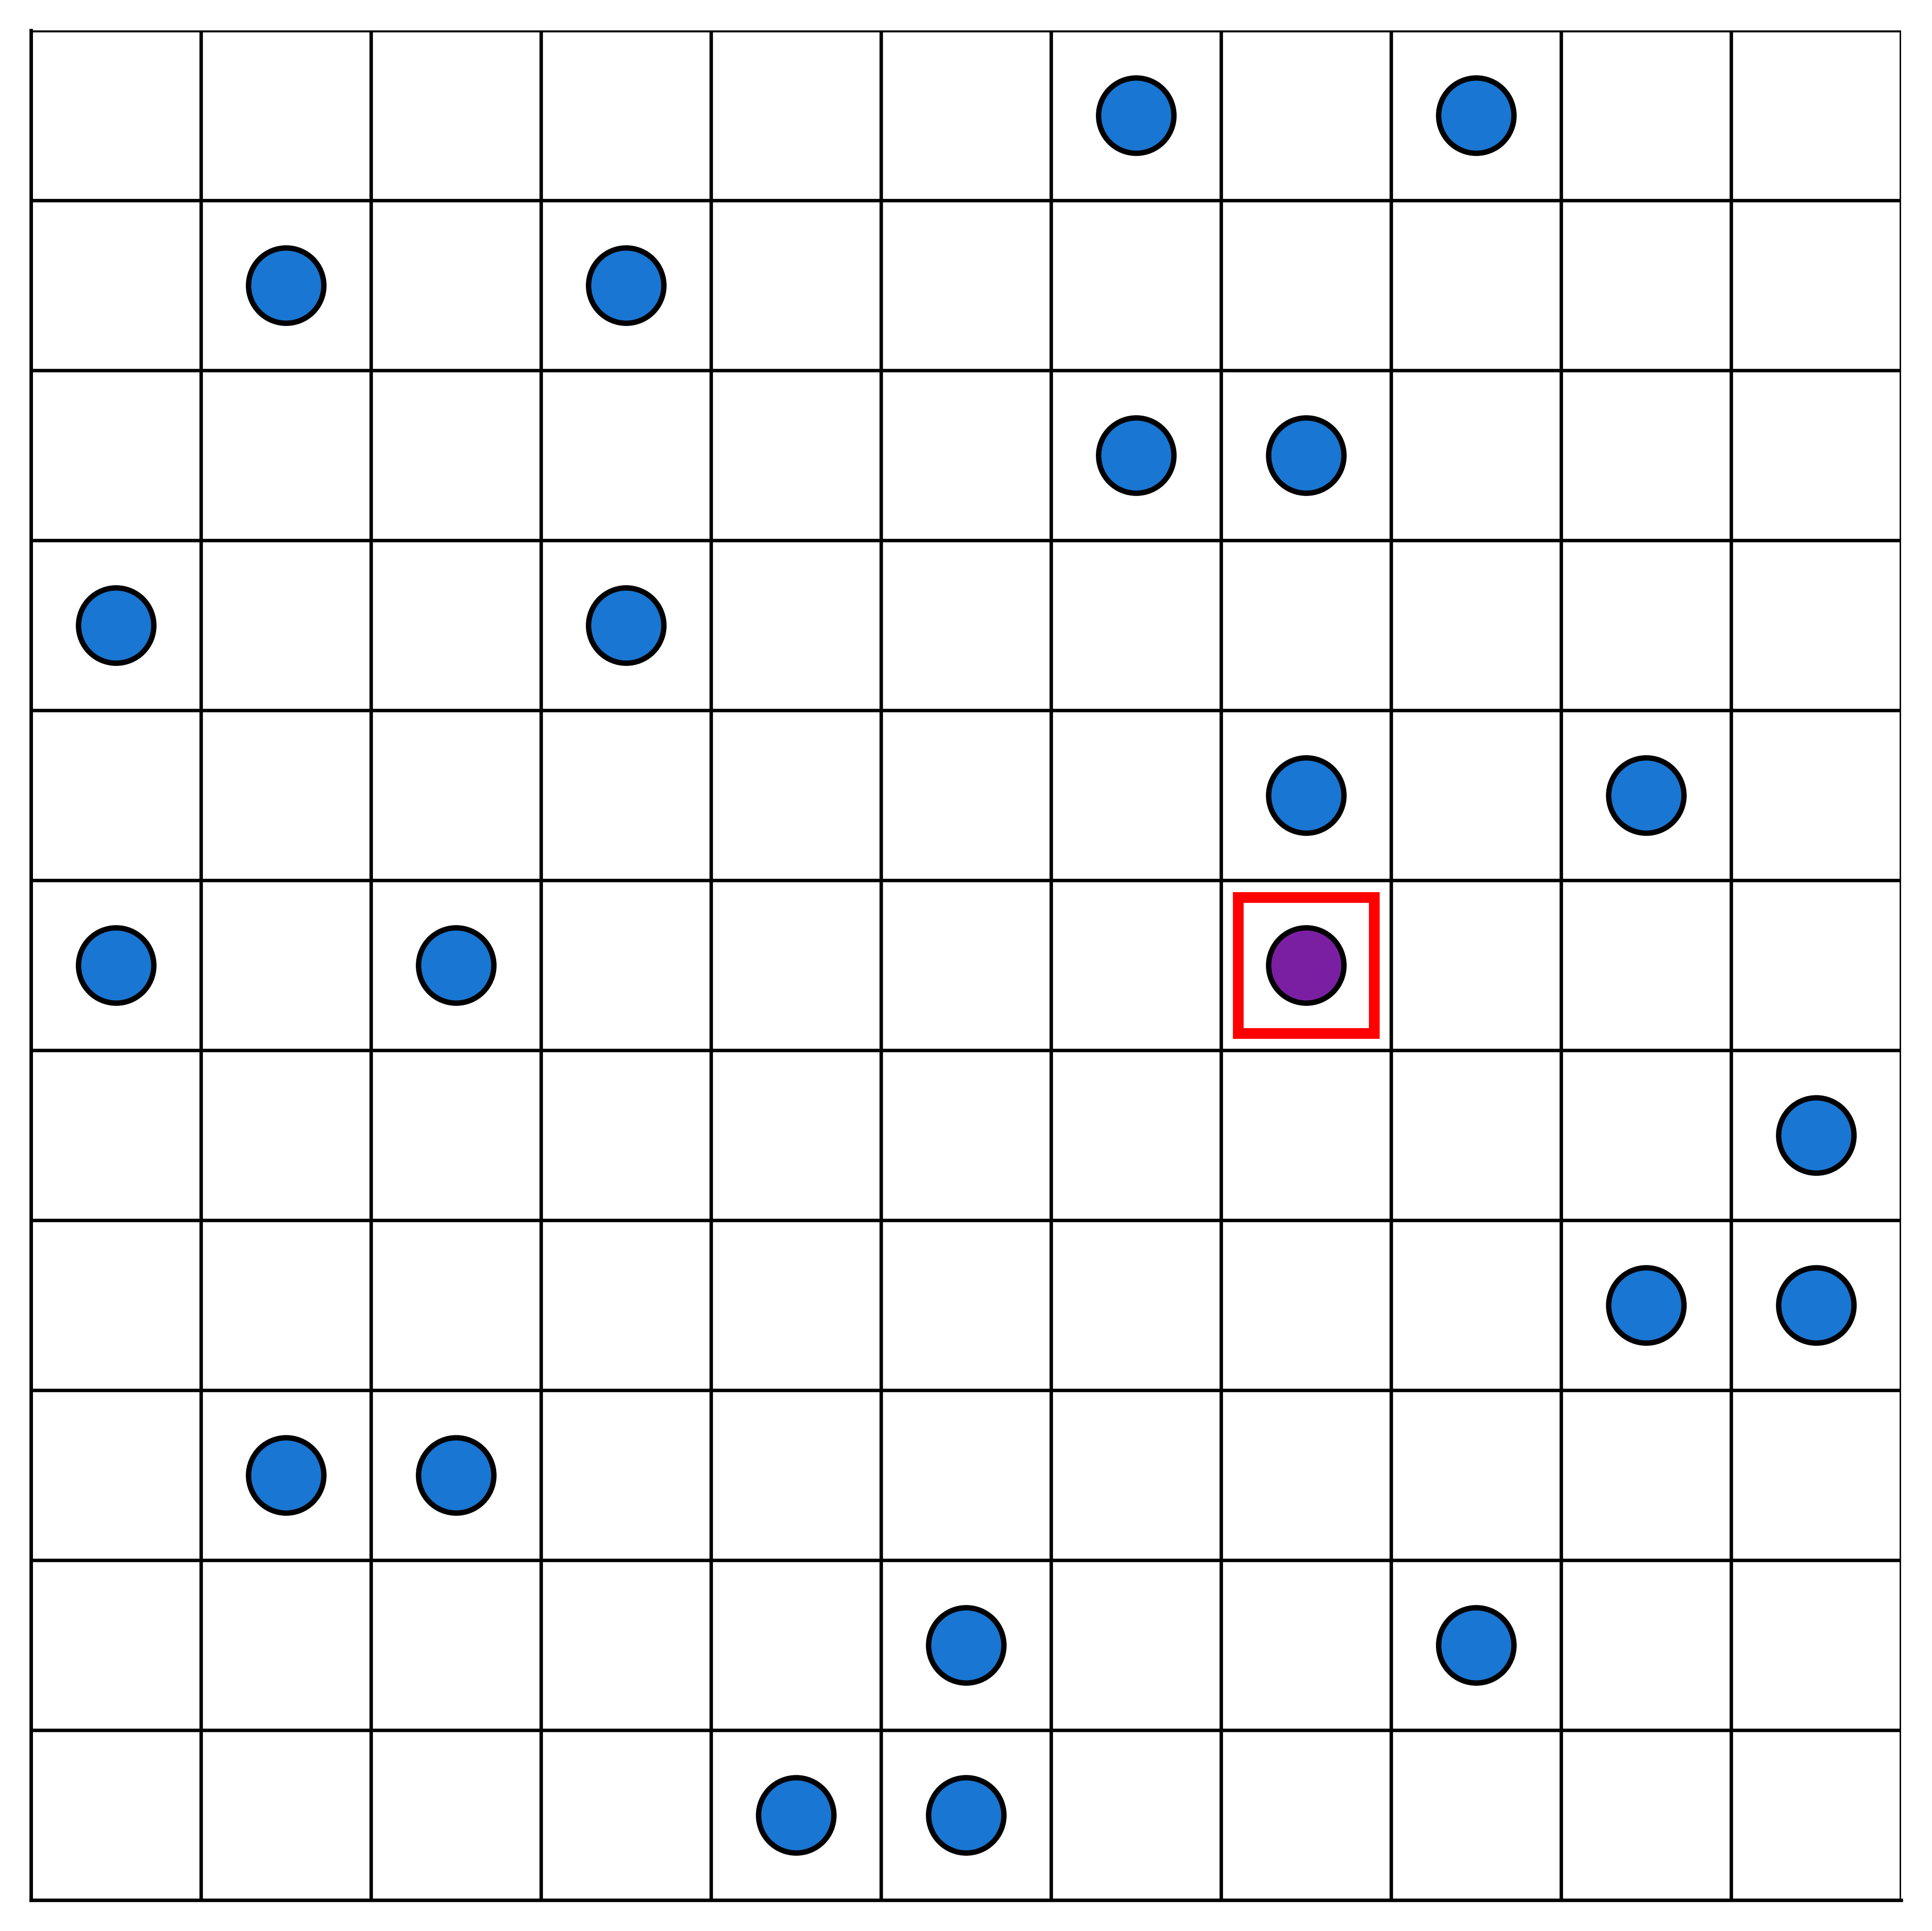
\includegraphics[width=\textwidth]{best_model_final_state_n11.png}
		\caption{PPO failure on $11 \times 11$ grid: 22 points with 1 violation.}
		\label{fig:rl_failure}
	\end{minipage}
	\hfill
	\begin{minipage}{0.48\textwidth}
		\centering
		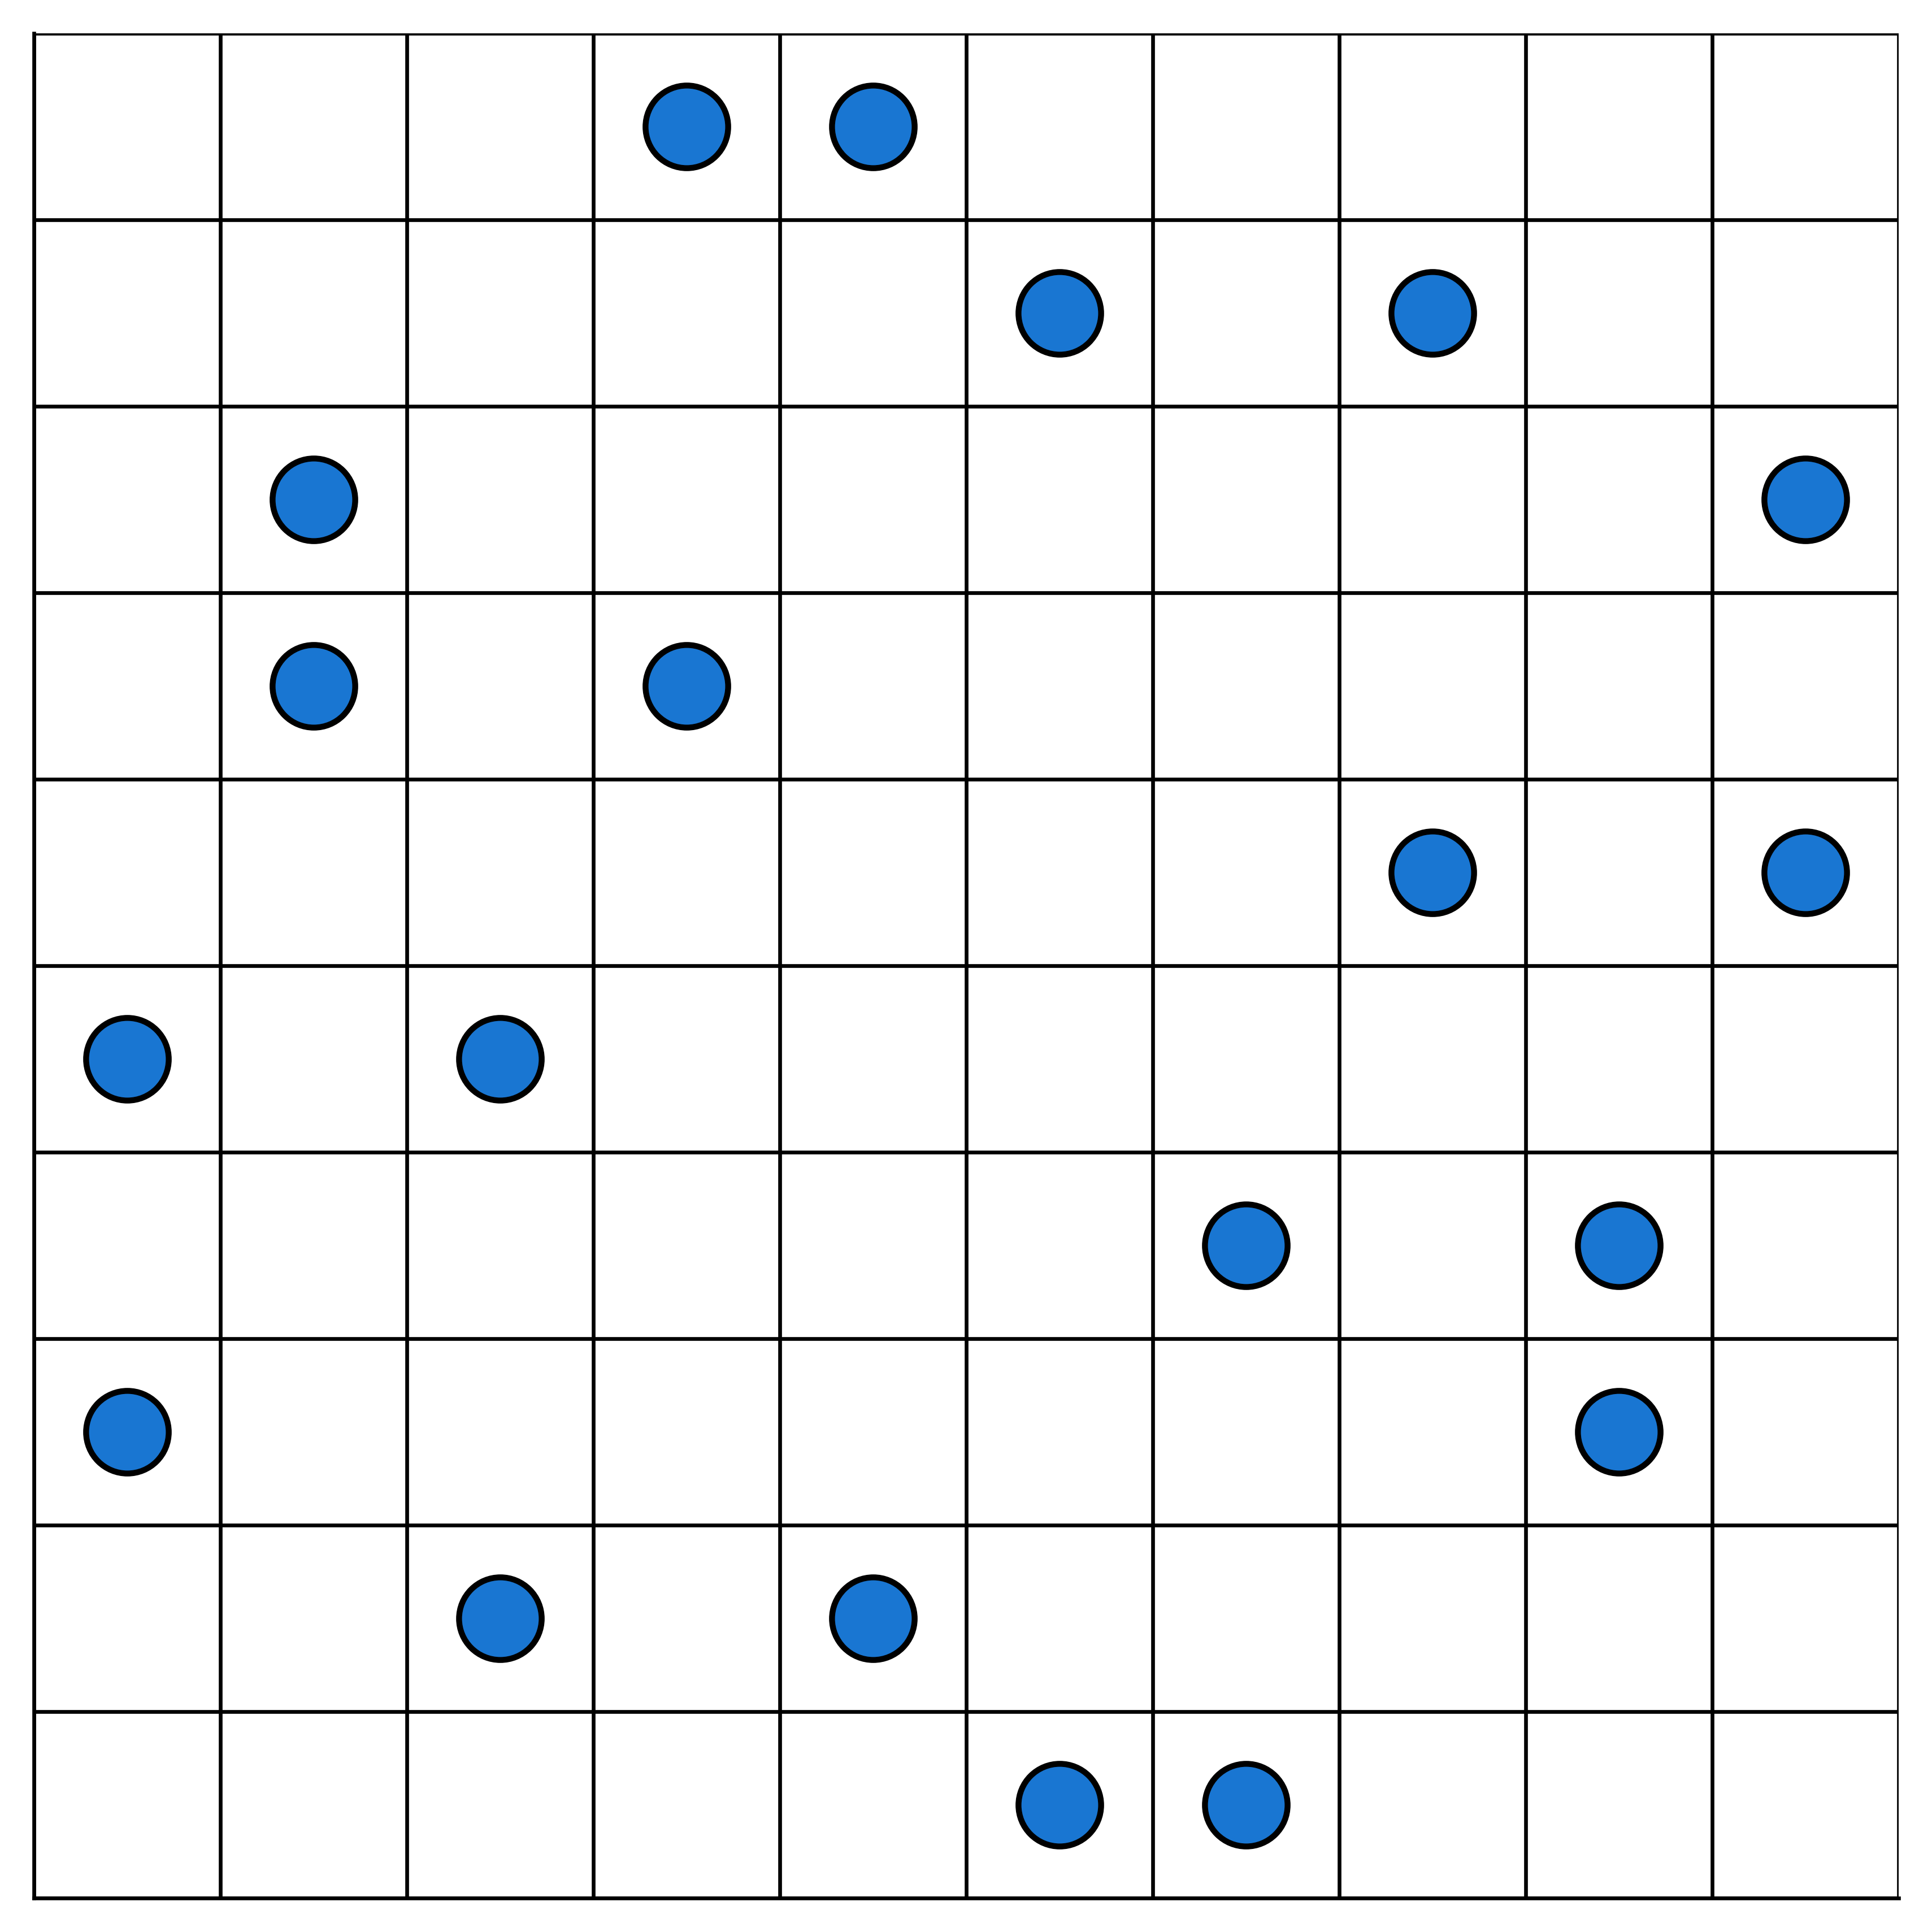
\includegraphics[width=\textwidth]{best_model_final_state_n10.png}
		\caption{PPO success on $10 \times 10$ grid: 20 points with 0 violations.}
		\label{fig:rl_success}
	\end{minipage}
\end{figure}

\begin{figure}[htbp]
		\centering
		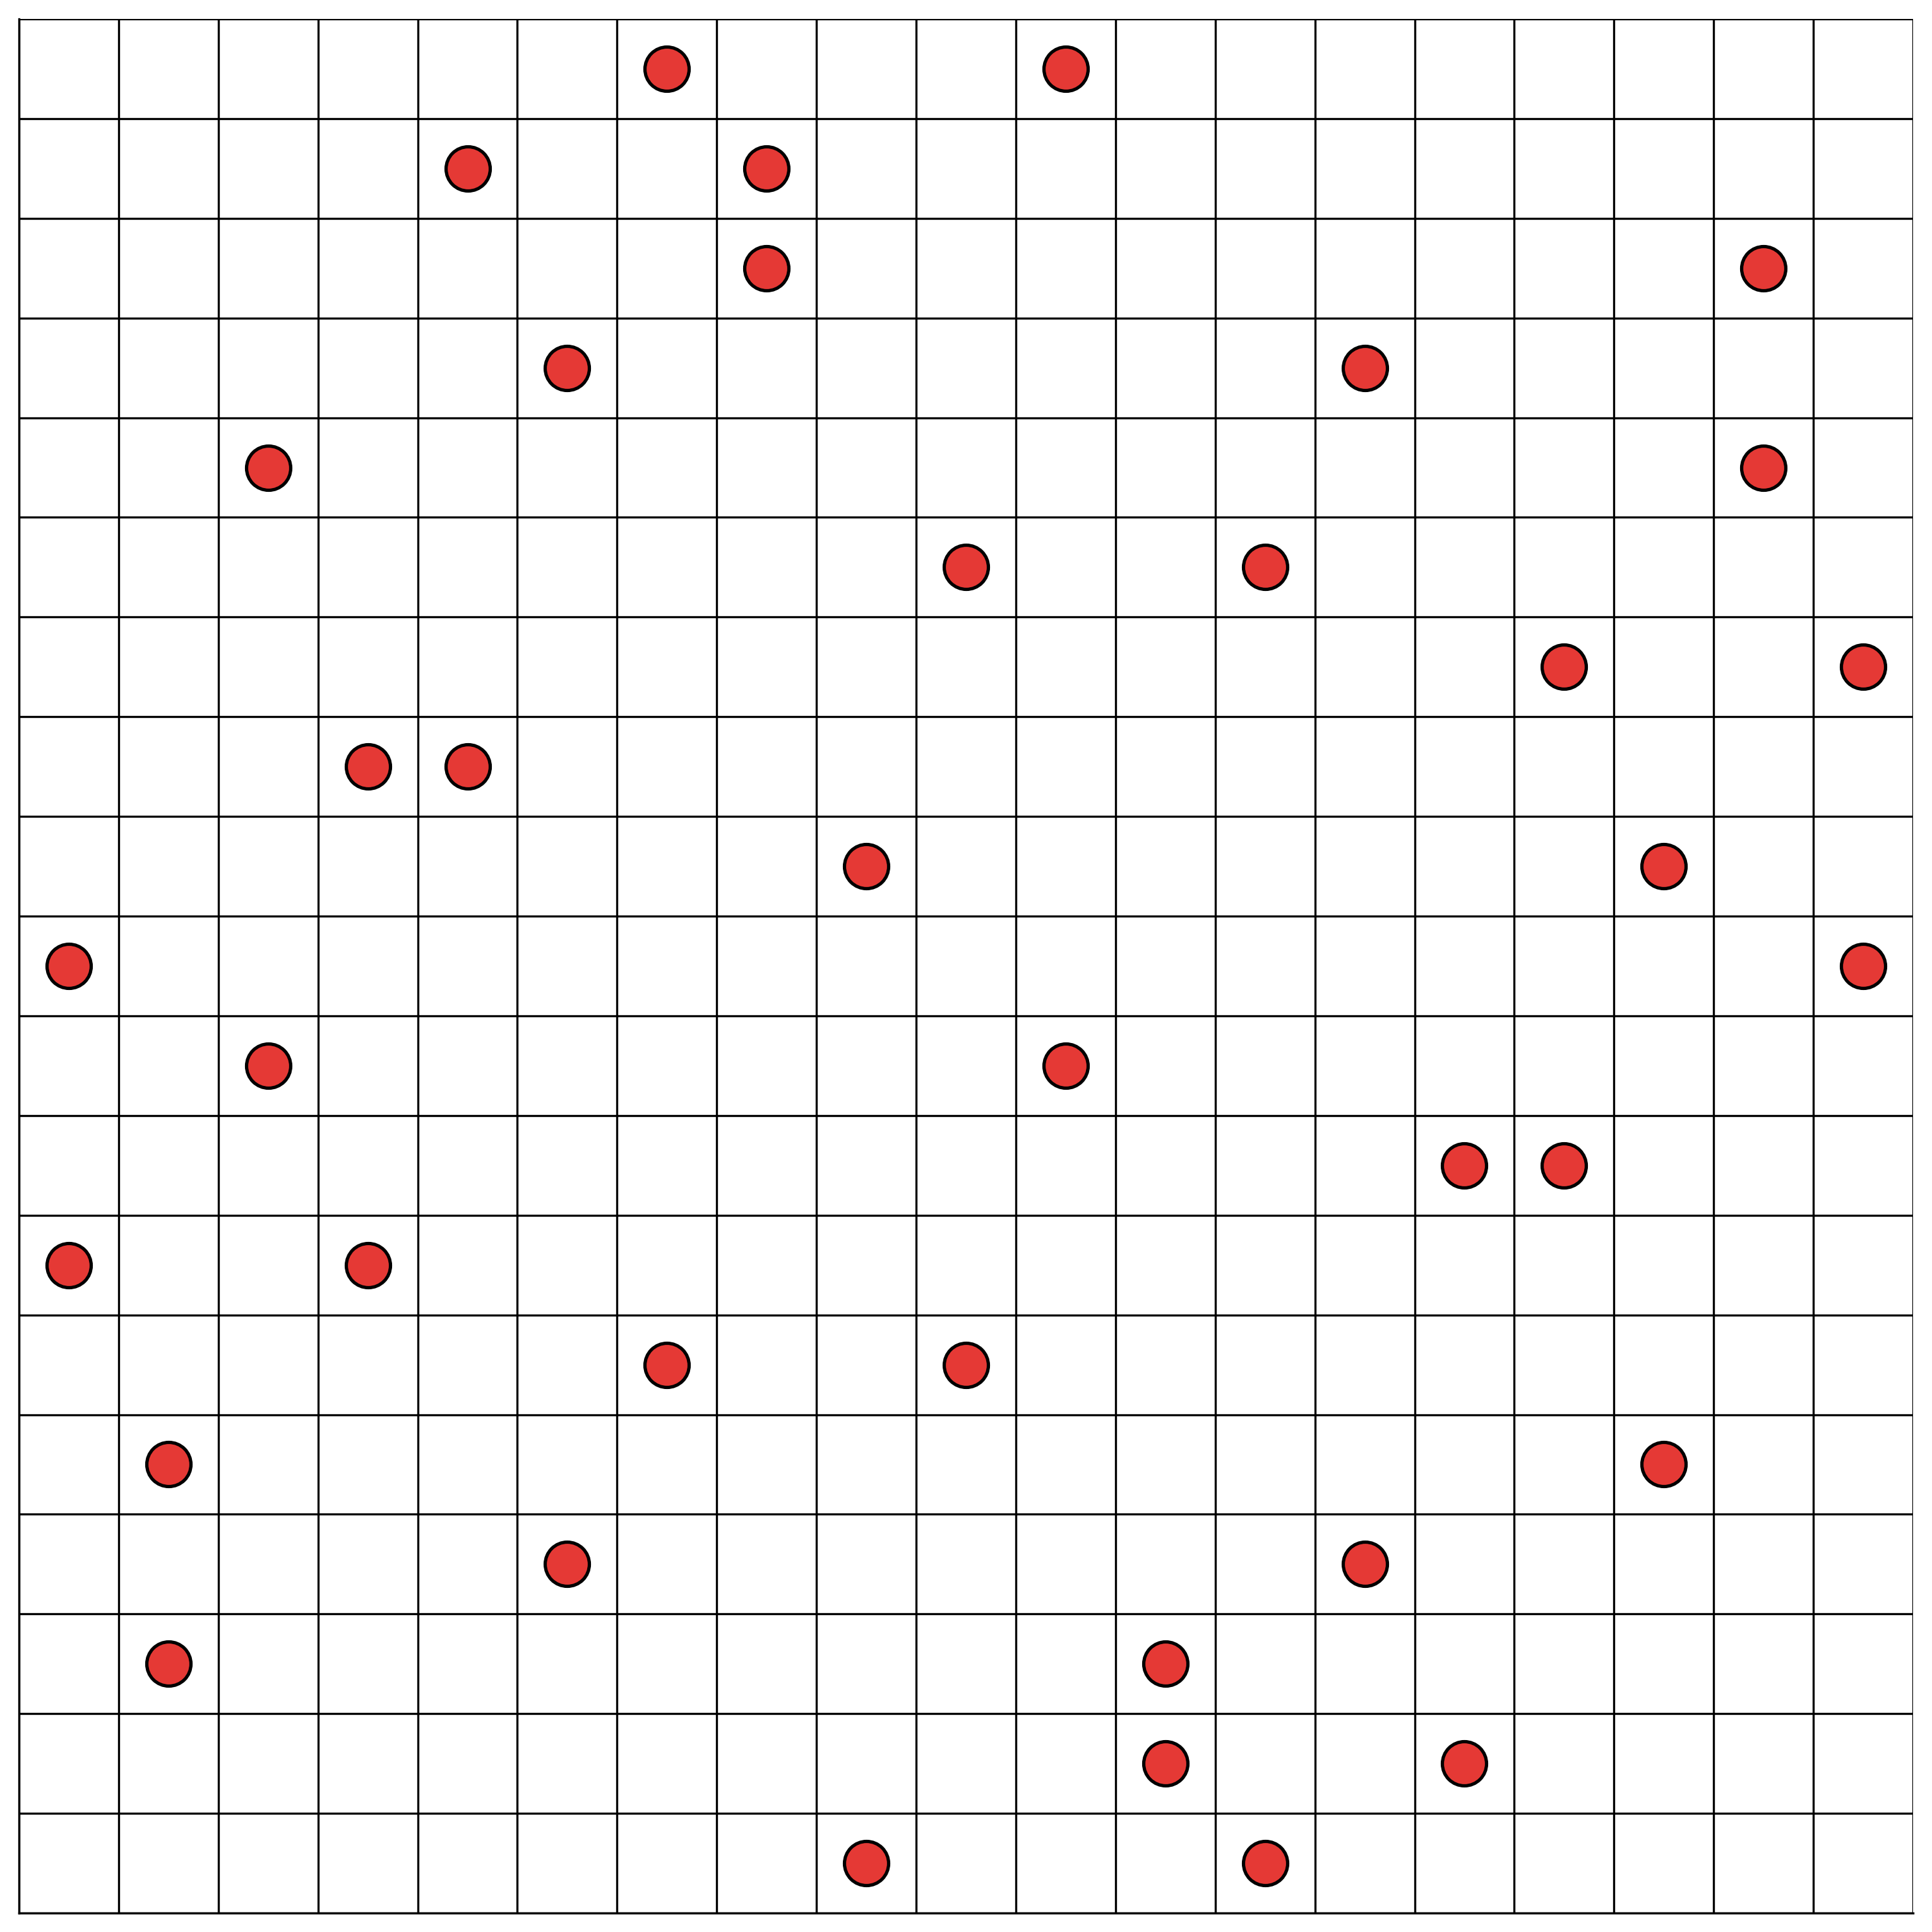
\includegraphics[width=\linewidth]{no_three_in_line_n19.png}
		\caption{ILP optimal solution on $19 \times 19$ grid achieving 38 points.}
		\label{fig:ilp_n19}
\end{figure}

\section{Discussion} % CHANGE (Frontiers): discussion section.

% TODO(SciML): Discussion augmentation, four additive insertions:
% (a) Para 1 thesis --- add SciML reach: optimal 2n up to n=18 on
%     Apple Metal without symmetry pruning, surpassing PatternBoost's
%     n=14 and PPO's n=10 ceilings. Reframe "first comparison of
%     classical optimization and AI approaches" -> "comparison of
%     classical, learning-based, and SciML approaches".
% (b) Para 2 trade-offs --- add SciML failure mode: continuous-discrete
%     gap at n=17 and n=19; Float32 GPU precision wall; threshold tau
%     sensitivity.
% (c) Para 3 limitations --- only Metal evaluated (no ROCm/CUDA cross-
%     validation); single-run hyperparameter regime per n; no symmetry
%     exploitation tried.
% (d) Para 4 future work (l. ~523, schuetz2022combinatorial cite) ---
%     pivot closing sentence to position SciML as the in-paper
%     instantiation of the physics-inspired direction, not just future
%     work.

Our study presents the first comparison of classical optimization and AI approaches to the No-Three-In-Line problem. Integer linear programming performed best, finding optimal solutions for up to $n = 19$, demonstrating the power of classical solvers for constraint satisfaction problems. In contrast, reinforcement learning approaches achieved perfect solutions only up to $n = 10$, with performance degrading by 42\% at $n = 11$ due to constraint violations. PatternBoost, the hybrid method combining classical greedy algorithms with transformers, achieved optimal solutions up to $n = 14$ and modest generalization to $n = 15$, bridging the gap between pure reinforcement learning and classical optimization. These findings underscore that hybrid approaches combining algorithmic heuristics with learned pattern recognition offer the most promising balance between solution quality and computational efficiency.

The distinct failure modes observed across methods reveal fundamental trade-offs in combinatorial optimization. ILP's branch-and-bound approach guarantees optimality through systematic search space pruning but faces exponential growth in problem complexity—constraints increased by 23\% from $n = 19$ (5,524 constraints) to $n = 20$ (6,778 constraints), illustrating the combinatorial explosion inherent to exact optimization. PatternBoost's philosophy of rapid training data generation through greedy algorithms creates a quality-speed trade-off: while fast data collection is central to the method's efficiency, the greedy approach struggles to find high-quality placements as problem complexity increases, constraining the quality of learned patterns. Reinforcement learning improved over training iterations but consistently produced constraint violations beyond $n = 10$, revealing fundamental difficulty in satisfying geometric constraints through reward-based exploration alone. These computational bottlenecks underscore that each method occupies a distinct niche in the optimization landscape.

This study is limited to grid sizes up to $n = 19$ for ILP, $n = 15$ for PatternBoost, and $n = 11$ for PPO, preventing definitive conclusions about asymptotic scaling behavior. We did not explore hybrid training combining supervised and reinforcement learning, transfer learning across grid sizes, or curriculum learning strategies that could leverage synergies between approaches. Computational constraints prevented exhaustive hyperparameter tuning and investigation of architectural improvements such as multi-branch networks or enhanced attention mechanisms for capturing long-range geometric dependencies. The PatternBoost model relies heavily on greedy-generated training data quality, with greedy algorithm limitations potentially propagating to the learned model. PPO's reward structure remains relatively simple and may benefit from more sophisticated shaping, intrinsic motivation signals, or exploration bonuses to better handle sparse binary rewards in constraint satisfaction tasks.

Future research should prioritize hybrid training paradigms that combine supervised pretraining (PatternBoost's cross-entropy learning) with reinforcement fine-tuning (PPO's exploratory optimization), mirroring successful approaches in language modeling. Transfer learning across grid sizes and curriculum strategies could enable training on smaller grids before scaling to larger instances, with meta-learning potentially discovering optimization strategies that generalize across problem scales. Classical-AI integration offers additional promising directions: ILP warm-starting with PatternBoost candidates could accelerate convergence on larger grids, while PatternBoost training on ILP-optimal smaller solutions could improve pattern quality beyond greedy baselines. Physics-inspired approaches present a particularly compelling direction, where combinatorial problems are reformulated as energy minimisation over relaxed Hamiltonians, enabling gradient-based neural network training~\cite{schuetz2022combinatorial}. 

% \section{Electronic Submission}

% Submission to ICML 2026 will be entirely electronic, via a web site
% (not email). Information about the submission process and \LaTeX\ templates
% are available on the conference web site at:
% \begin{center}
%   \texttt{http://icml.cc/}
% \end{center}

% The guidelines below will be enforced for initial submissions and
% camera-ready copies. Here is a brief summary:
% \begin{itemize}
%   \item Submissions must be in PDF\@.
%   \item If your paper has appendices, submit the appendix together with the
%         main body and the references \textbf{as a single file}. Reviewers will not
%         look for appendices as a separate PDF file. So if you submit such an extra
%         file, reviewers will very likely miss it.
%   \item Page limit: The main body of the paper has to be fitted to 8 pages,
%         excluding references and appendices; the space for the latter two is not
%         limited in pages, but the total file size may not exceed 10MB. For the
%         final version of the paper, authors can add one extra page to the main
%         body.
%   \item \textbf{Do not include author information or acknowledgements} in your
%         initial submission.
%   \item Your paper should be in \textbf{10 point Times font}.
%   \item Make sure your PDF file only uses Type-1 fonts.
%   \item Place figure captions \emph{under} the figure (and omit titles from
%         inside the graphic file itself). Place table captions \emph{over} the
%         table.
%   \item References must include page numbers whenever possible and be as
%         complete as possible. Place multiple citations in chronological order.
%   \item Do not alter the style template; in particular, do not compress the
%         paper format by reducing the vertical spaces.
%   \item Keep your abstract brief and self-contained, one paragraph and roughly
%         4--6 sentences. Gross violations will require correction at the
%         camera-ready phase. The title should have content words capitalized.
% \end{itemize}

% \subsection{Submitting Papers}

% \textbf{Anonymous Submission:} ICML uses double-blind review: no identifying
% author information may appear on the title page or in the paper
% itself. \cref{author info} gives further details.

% \medskip

% Authors must provide their manuscripts in \textbf{PDF} format.
% Furthermore, please make sure that files contain only embedded Type-1 fonts
% (e.g.,~using the program \texttt{pdffonts} in linux or using
% File/DocumentProperties/Fonts in Acrobat). Other fonts (like Type-3)
% might come from graphics files imported into the document.

% Authors using \textbf{Word} must convert their document to PDF\@. Most
% of the latest versions of Word have the facility to do this
% automatically. Submissions will not be accepted in Word format or any
% format other than PDF\@. Really. We're not joking. Don't send Word.

% Those who use \textbf{\LaTeX} should avoid including Type-3 fonts.
% Those using \texttt{latex} and \texttt{dvips} may need the following
% two commands:

% {\footnotesize
% \begin{verbatim}
% dvips -Ppdf -tletter -G0 -o paper.ps paper.dvi
% ps2pdf paper.ps
% \end{verbatim}}
% It is a zero following the ``-G'', which tells dvips to use
% the config.pdf file. Newer \TeX\ distributions don't always need this
% option.

% Using \texttt{pdflatex} rather than \texttt{latex}, often gives better
% results. This program avoids the Type-3 font problem, and supports more
% advanced features in the \texttt{microtype} package.

% \textbf{Graphics files} should be a reasonable size, and included from
% an appropriate format. Use vector formats (.eps/.pdf) for plots,
% lossless bitmap formats (.png) for raster graphics with sharp lines, and
% jpeg for photo-like images.

% The style file uses the \texttt{hyperref} package to make clickable
% links in documents. If this causes problems for you, add
% \texttt{nohyperref} as one of the options to the \texttt{icml2026}
% usepackage statement.

% \subsection{Submitting Final Camera-Ready Copy}

% The final versions of papers accepted for publication should follow the
% same format and naming convention as initial submissions, except that
% author information (names and affiliations) should be given. See
% \cref{final author} for formatting instructions.

% The footnote, ``Preliminary work. Under review by the International
% Conference on Machine Learning (ICML). Do not distribute.'' must be
% modified to ``\textit{Proceedings of the
%   $\mathit{43}^{rd}$ International Conference on Machine Learning},
% Seoul, South Korea, PMLR 306, 2026.
% Copyright 2026 by the author(s).''

% For those using the \textbf{\LaTeX} style file, this change (and others) is
% handled automatically by simply changing
% $\mathtt{\backslash usepackage\{icml2026\}}$ to
% $$\mathtt{\backslash usepackage[accepted]\{icml2026\}}$$
% Authors using \textbf{Word} must edit the
% footnote on the first page of the document themselves.

% Camera-ready copies should have the title of the paper as running head
% on each page except the first one. The running title consists of a
% single line centered above a horizontal rule which is $1$~point thick.
% The running head should be centered, bold and in $9$~point type. The
% rule should be $10$~points above the main text. For those using the
% \textbf{\LaTeX} style file, the original title is automatically set as running
% head using the \texttt{fancyhdr} package which is included in the ICML
% 2026 style file package. In case that the original title exceeds the
% size restrictions, a shorter form can be supplied by using

% \verb|\icmltitlerunning{...}|

% just before $\mathtt{\backslash begin\{document\}}$.
% Authors using \textbf{Word} must edit the header of the document themselves.

% \section{Format of the Paper}

% All submissions must follow the specified format.

% \subsection{Dimensions}

% The text of the paper should be formatted in two columns, with an
% overall width of 6.75~inches, height of 9.0~inches, and 0.25~inches
% between the columns. The left margin should be 0.75~inches and the top
% margin 1.0~inch (2.54~cm). The right and bottom margins will depend on
% whether you print on US letter or A4 paper, but all final versions
% must be produced for US letter size.
% Do not write anything on the margins.

% The paper body should be set in 10~point type with a vertical spacing
% of 11~points. Please use Times typeface throughout the text.

% \subsection{Title}

% The paper title should be set in 14~point bold type and centered
% between two horizontal rules that are 1~point thick, with 1.0~inch
% between the top rule and the top edge of the page. Capitalize the
% first letter of content words and put the rest of the title in lower
% case.
% You can use TeX math in the title (we suggest sparingly),
% but no custom macros, images, or other TeX commands.
% Please make sure that accents, special characters, etc., are entered using
% TeX commands and not using non-English characters.

% \subsection{Author Information for Submission}
% \label{author info}

% ICML uses double-blind review, so author information must not appear. If
% you are using \LaTeX\/ and the \texttt{icml2026.sty} file, use
% \verb+\icmlauthor{...}+ to specify authors and \verb+\icmlaffiliation{...}+
% to specify affiliations. (Read the TeX code used to produce this document for
% an example usage.) The author information will not be printed unless
% \texttt{accepted} is passed as an argument to the style file. Submissions that
% include the author information will not be reviewed.

% \subsubsection{Self-Citations}

% If you are citing published papers for which you are an author, refer
% to yourself in the third person. In particular, do not use phrases
% that reveal your identity (e.g., ``in previous work \cite{langley00}, we
% have shown \ldots'').

% Do not anonymize citations in the reference section. The only exception are manuscripts that are
% not yet published (e.g., under submission). If you choose to refer to
% such unpublished manuscripts \cite{anonymous}, anonymized copies have
% to be submitted
% as Supplementary Material via OpenReview\@. However, keep in mind that an ICML
% paper should be self contained and should contain sufficient detail
% for the reviewers to evaluate the work. In particular, reviewers are
% not required to look at the Supplementary Material when writing their
% review (they are not required to look at more than the first $8$ pages of the submitted document).

% \subsubsection{Camera-Ready Author Information}
% \label{final author}

% If a paper is accepted, a final camera-ready copy must be prepared.
% %
% For camera-ready papers, author information should start 0.3~inches below the
% bottom rule surrounding the title. The authors' names should appear in 10~point
% bold type, in a row, separated by white space, and centered. Author names should
% not be broken across lines. Unbolded superscripted numbers, starting 1, should
% be used to refer to affiliations.

% Affiliations should be numbered in the order of appearance. A single footnote
% block of text should be used to list all the affiliations. (Academic
% affiliations should list Department, University, City, State/Region, Country.
% Similarly for industrial affiliations.)

% Each distinct affiliations should be listed once. If an author has multiple
% affiliations, multiple superscripts should be placed after the name, separated
% by thin spaces. If the authors would like to highlight equal contribution by
% multiple first authors, those authors should have an asterisk placed after their
% name in superscript, and the term ``\textsuperscript{*}Equal contribution"
% should be placed in the footnote block ahead of the list of affiliations. A
% list of corresponding authors and their emails (in the format Full Name
% \textless{}email@domain.com\textgreater{}) can follow the list of affiliations.
% Ideally only one or two names should be listed.

% A sample file with author names is included in the ICML2026 style file
% package. Turn on the \texttt{[accepted]} option to the stylefile to
% see the names rendered. All of the guidelines above are implemented
% by the \LaTeX\ style file.

% \subsection{Abstract}

% The paper abstract should begin in the left column, 0.4~inches below the final
% address. The heading `Abstract' should be centered, bold, and in 11~point type.
% The abstract body should use 10~point type, with a vertical spacing of
% 11~points, and should be indented 0.25~inches more than normal on left-hand and
% right-hand margins. Insert 0.4~inches of blank space after the body. Keep your
% abstract brief and self-contained, limiting it to one paragraph and roughly 4--6
% sentences. Gross violations will require correction at the camera-ready phase.

% \subsection{Partitioning the Text}

% You should organize your paper into sections and paragraphs to help readers
% place a structure on the material and understand its contributions.

% \subsubsection{Sections and Subsections}

% Section headings should be numbered, flush left, and set in 11~pt bold type
% with the content words capitalized. Leave 0.25~inches of space before the
% heading and 0.15~inches after the heading.

% Similarly, subsection headings should be numbered, flush left, and set in 10~pt
% bold type with the content words capitalized. Leave
% 0.2~inches of space before the heading and 0.13~inches afterward.

% Finally, subsubsection headings should be numbered, flush left, and set in
% 10~pt small caps with the content words capitalized. Leave
% 0.18~inches of space before the heading and 0.1~inches after the heading.

% Please use no more than three levels of headings.

% \subsubsection{Paragraphs and Footnotes}

% Within each section or subsection, you should further partition the paper into
% paragraphs. Do not indent the first line of a given paragraph, but insert a
% blank line between succeeding ones.

% You can use footnotes\footnote{Footnotes should be complete sentences.}
% to provide readers with additional information about a topic without
% interrupting the flow of the paper. Indicate footnotes with a number in the
% text where the point is most relevant. Place the footnote in 9~point type at
% the bottom of the column in which it appears. Precede the first footnote in a
% column with a horizontal rule of 0.8~inches.\footnote{Multiple footnotes can
%   appear in each column, in the same order as they appear in the text,
%   but spread them across columns and pages if possible.}

% \begin{figure}[ht]
%   \vskip 0.2in
%   \begin{center}
%     \centerline{
\includegraphics[width=\columnwidth]{icml_numpapers}}
%     \caption{
%       Historical locations and number of accepted papers for International
%       Machine Learning Conferences (ICML 1993 -- ICML 2008) and International
%       Workshops on Machine Learning (ML 1988 -- ML 1992). At the time this
%       figure was produced, the number of accepted papers for ICML 2008 was
%       unknown and instead estimated.
%     }
%     \label{icml-historical}
%   \end{center}
% \end{figure}

% \subsection{Figures}

% You may want to include figures in the paper to illustrate your approach and
% results. Such artwork should be centered, legible, and separated from the text.
% Lines should be dark and at least 0.5~points thick for purposes of
% reproduction, and text should not appear on a gray background.

% Label all distinct components of each figure. If the figure takes the form of a
% graph, then give a name for each axis and include a legend that briefly
% describes each curve. Do not include a title inside the figure; instead, the
% caption should serve this function.

% Number figures sequentially, placing the figure number and caption \emph{after}
% the graphics, with at least 0.1~inches of space before the caption and
% 0.1~inches after it, as in \cref{icml-historical}. The figure caption should be
% set in 9~point type and centered unless it runs two or more lines, in which
% case it should be flush left. You may float figures to the top or bottom of a
% column, and you may set wide figures across both columns (use the environment
% \texttt{figure*} in \LaTeX). Always place two-column figures at the top or
% bottom of the page.

% \subsection{Algorithms}

% If you are using \LaTeX, please use the ``algorithm'' and ``algorithmic''
% environments to format pseudocode. These require the corresponding stylefiles,
% algorithm.sty and algorithmic.sty, which are supplied with this package.
% \cref{alg:example} shows an example.

% \begin{algorithm}[tb]
%   \caption{Bubble Sort}
%   \label{alg:example}
%   \begin{algorithmic}
%     \STATE {\bfseries Input:} data $x_i$, size $m$
%     \REPEAT
%     \STATE Initialize $noChange = true$.
%     \FOR{$i=1$ {\bfseries to} $m-1$}
%     \IF{$x_i > x_{i+1}$}
%     \STATE Swap $x_i$ and $x_{i+1}$
%     \STATE $noChange = false$
%     \ENDIF
%     \ENDFOR
%     \UNTIL{$noChange$ is $true$}
%   \end{algorithmic}
% \end{algorithm}


% \subsection{Tables}

% You may also want to include tables that summarize material. Like figures,
% these should be centered, legible, and numbered consecutively. However, place
% the title \emph{above} the table with at least 0.1~inches of space before the
% title and the same after it, as in \cref{sample-table}. The table title should
% be set in 9~point type and centered unless it runs two or more lines, in which
% case it should be flush left.

% % Note use of \abovespace and \belowspace to get reasonable spacing
% % above and below tabular lines.

% \begin{table}[t]
%   \caption{Classification accuracies for naive Bayes and flexible
%     Bayes on various data sets.}
%   \label{sample-table}
%   \begin{center}
%     \begin{small}
%       \begin{sc}
%         \begin{tabular}{lcccr}
%           \toprule
%           Data set  & Naive         & Flexible      & Better?  \\
%           \midrule
%           Breast    & 95.9$\pm$ 0.2 & 96.7$\pm$ 0.2 & $\surd$  \\
%           Cleveland & 83.3$\pm$ 0.6 & 80.0$\pm$ 0.6 & $\times$ \\
%           Glass2    & 61.9$\pm$ 1.4 & 83.8$\pm$ 0.7 & $\surd$  \\
%           Credit    & 74.8$\pm$ 0.5 & 78.3$\pm$ 0.6 &          \\
%           Horse     & 73.3$\pm$ 0.9 & 69.7$\pm$ 1.0 & $\times$ \\
%           Meta      & 67.1$\pm$ 0.6 & 76.5$\pm$ 0.5 & $\surd$  \\
%           Pima      & 75.1$\pm$ 0.6 & 73.9$\pm$ 0.5 &          \\
%           Vehicle   & 44.9$\pm$ 0.6 & 61.5$\pm$ 0.4 & $\surd$  \\
%           \bottomrule
%         \end{tabular}
%       \end{sc}
%     \end{small}
%   \end{center}
%   \vskip -0.1in
% \end{table}

% Tables contain textual material, whereas figures contain graphical material.
% Specify the contents of each row and column in the table's topmost row. Again,
% you may float tables to a column's top or bottom, and set wide tables across
% both columns. Place two-column tables at the top or bottom of the page.

% \subsection{Theorems and Such}
% The preferred way is to number definitions, propositions, lemmas, etc.
% consecutively, within sections, as shown below.
% \begin{definition}
%   \label{def:inj}
%   A function $f:X \to Y$ is injective if for any $x,y\in X$ different, $f(x)\ne
%     f(y)$.
% \end{definition}
% Using \cref{def:inj} we immediate get the following result:
% \begin{proposition}
%   If $f$ is injective mapping a set $X$ to another set $Y$,
%   the cardinality of $Y$ is at least as large as that of $X$
% \end{proposition}
% \begin{proof}
%   Left as an exercise to the reader.
% \end{proof}
% \cref{lem:usefullemma} stated next will prove to be useful.
% \begin{lemma}
%   \label{lem:usefullemma}
%   For any $f:X \to Y$ and $g:Y\to Z$ injective functions, $f \circ g$ is
%   injective.
% \end{lemma}
% \begin{theorem}
%   \label{thm:bigtheorem}
%   If $f:X\to Y$ is bijective, the cardinality of $X$ and $Y$ are the same.
% \end{theorem}
% An easy corollary of \cref{thm:bigtheorem} is the following:
% \begin{corollary}
%   If $f:X\to Y$ is bijective,
%   the cardinality of $X$ is at least as large as that of $Y$.
% \end{corollary}
% \begin{assumption}
%   The set $X$ is finite.
%   \label{ass:xfinite}
% \end{assumption}
% \begin{remark}
%   According to some, it is only the finite case (cf. \cref{ass:xfinite}) that
%   is interesting.
% \end{remark}
%restatable

% \subsection{Citations and References}

% Please use APA reference format regardless of your formatter or word processor.
% If you rely on the \LaTeX\/ bibliographic facility, use \texttt{natbib.sty} and
% \texttt{icml2026.bst} included in the style-file package to obtain this format.

% Citations within the text should include the authors' last names and year. If
% the authors' names are included in the sentence, place only the year in
% parentheses, for example when referencing Arthur Samuel's pioneering work
% \yrcite{Samuel59}. Otherwise place the entire reference in parentheses with the
% authors and year separated by a comma \cite{Samuel59}. List multiple references
% separated by semicolons \cite{kearns89,Samuel59,mitchell80}. Use the `et~al.'
% construct only for citations with three or more authors or after listing all
% authors to a publication in an earlier reference \cite{MachineLearningI}.

% Authors should cite their own work in the third person in the initial version
% of their paper submitted for blind review. Please refer to \cref{author info}
% for detailed instructions on how to cite your own papers.

% Use an unnumbered first-level section heading for the references, and use a
% hanging indent style, with the first line of the reference flush against the
% left margin and subsequent lines indented by 10 points. The references at the
% end of this document give examples for journal articles \cite{Samuel59},
% conference publications \cite{langley00}, book chapters \cite{Newell81}, books
% \cite{DudaHart2nd}, edited volumes \cite{MachineLearningI}, technical reports
% \cite{mitchell80}, and dissertations \cite{kearns89}.

% Alphabetize references by the surnames of the first authors, with single author
% entries preceding multiple author entries. Order references for the same
% authors by year of publication, with the earliest first. Make sure that each
% reference includes all relevant information (e.g., page numbers).

% Please put some effort into making references complete, presentable, and
% consistent, e.g. use the actual current name of authors. If using bibtex,
% please protect capital letters of names and abbreviations in titles, for
% example, use \{B\}ayesian or \{L\}ipschitz in your .bib file.

% \section*{Accessibility}

% Authors are kindly asked to make their submissions as accessible as possible
% for everyone including people with disabilities and sensory or neurological
% differences. Tips of how to achieve this and what to pay attention to will be
% provided on the conference website \url{http://icml.cc/}.

\section*{Software and Data}

% TODO(SciML): change "all three methods" to "all four methods" once
% the SciML repo URL bullet below is filled in.
The code for all three methods is available in the following repositories:

\begin{itemize}
    \item ILP: \url{https://github.com/pranav-ramanathan/N3L_gurobi}
    \item PatternBoost: \url{https://github.com/pranav-ramanathan/N3L_PatternBoost}
    \item RL: \url{https://github.com/pranav-ramanathan/N3L_RL}
    \item SciML: % TODO(SciML): public repo URL or "available on request".
\end{itemize}

% If a paper is accepted, we strongly encourage the publication of software and
% data with the camera-ready version of the paper whenever appropriate. This can
% be done by including a URL in the camera-ready copy. However, \textbf{do not}
% include URLs that reveal your institution or identity in your submission for
% review. Instead, provide an anonymous URL or upload the material as
% ``Supplementary Material'' into the OpenReview reviewing system. Note that
% reviewers are not required to look at this material when writing their review.

% % Acknowledgements should only appear in the accepted version.
% \section*{Acknowledgements}

% \textbf{Do not} include acknowledgements in the initial version of the paper
% submitted for blind review.

% If a paper is accepted, the final camera-ready version can (and usually should)
% include acknowledgements.  Such acknowledgements should be placed at the end of
% the section, in an unnumbered section that does not count towards the paper
% page limit. Typically, this will include thanks to reviewers who gave useful
% comments, to colleagues who contributed to the ideas, and to funding agencies
% and corporate sponsors that provided financial support.

\section*{Impact Statement}

Authors are \textbf{required} to include a statement of the potential broader
impact of their work, including its ethical aspects and future societal
consequences. This statement should be in an unnumbered section at the end of
the paper (co-located with Acknowledgements -- the two may appear in either
order, but both must be before References), and does not count toward the paper
page limit. In many cases, where the ethical impacts and expected societal
implications are those that are well established when advancing the field of
Machine Learning, substantial discussion is not required, and a simple
statement such as the following will suffice:

``This paper presents work whose goal is to advance the field of Machine
Learning. There are many potential societal consequences of our work, none
which we feel must be specifically highlighted here.''

The above statement can be used verbatim in such cases, but we encourage
authors to think about whether there is content which does warrant further
discussion, as this statement will be apparent if the paper is later flagged
for ethics review.

\bibliography{main}
\bibliographystyle{icml2026}

%%%%%%%%%%%%%%%%%%%%%%%%%%%%%%%%%%%%%%%%%%%%%%%%%%%%%%%%%%%%%%%%%%%%%%%%%%%%%%%
%%%%%%%%%%%%%%%%%%%%%%%%%%%%%%%%%%%%%%%%%%%%%%%%%%%%%%%%%%%%%%%%%%%%%%%%%%%%%%%
% APPENDIX
%%%%%%%%%%%%%%%%%%%%%%%%%%%%%%%%%%%%%%%%%%%%%%%%%%%%%%%%%%%%%%%%%%%%%%%%%%%%%%%
%%%%%%%%%%%%%%%%%%%%%%%%%%%%%%%%%%%%%%%%%%%%%%%%%%%%%%%%%%%%%%%%%%%%%%%%%%%%%%%
\newpage
\appendix
\onecolumn
\section{You \emph{can} have an appendix here.}

You can have as much text here as you want. The main body must be at most $8$
pages long. For the final version, one more page can be added. If you want, you
can use an appendix like this one.

The $\mathtt{\backslash onecolumn}$ command above can be kept in place if you
prefer a one-column appendix, or can be removed if you prefer a two-column
appendix.  Apart from this possible change, the style (font size, spacing,
margins, page numbering, etc.) should be kept the same as the main body.
%%%%%%%%%%%%%%%%%%%%%%%%%%%%%%%%%%%%%%%%%%%%%%%%%%%%%%%%%%%%%%%%%%%%%%%%%%%%%%%
%%%%%%%%%%%%%%%%%%%%%%%%%%%%%%%%%%%%%%%%%%%%%%%%%%%%%%%%%%%%%%%%%%%%%%%%%%%%%%%

\end{document}
